\documentclass[a4paper]{article}

\def\npart{IB}

\def\ntitle{Analysis II}
\def\nlecturer{J.\ Rasmussen}

\def\nterm{Michaelmas}
\def\nyear{2017}

\ifx \nauthor\undefined
  \def\nauthor{Qiangru Kuang}
\else
\fi

\ifx \ntitle\undefined
  \def\ntitle{Template}
\else
\fi

\ifx \nauthoremail\undefined
  \def\nauthoremail{qk206@cam.ac.uk}
\else
\fi

\ifx \ndate\undefined
  \def\ndate{\today}
\else
\fi

\title{\ntitle}
\author{\nauthor}
\date{\ndate}

%\usepackage{microtype}
\usepackage{mathtools}
\usepackage{amsthm}
\usepackage{stmaryrd}%symbols used so far: \mapsfrom
\usepackage{empheq}
\usepackage{amssymb}
\let\mathbbalt\mathbb
\let\pitchforkold\pitchfork
\usepackage{unicode-math}
\let\mathbb\mathbbalt%reset to original \mathbb
\let\pitchfork\pitchforkold

\usepackage{imakeidx}
\makeindex[intoc]

%to address the problem that Latin modern doesn't have unicode support for setminus
%https://tex.stackexchange.com/a/55205/26707
\AtBeginDocument{\renewcommand*{\setminus}{\mathbin{\backslash}}}
\AtBeginDocument{\renewcommand*{\models}{\vDash}}%for \vDash is same size as \vdash but orginal \models is larger
\AtBeginDocument{\let\Re\relax}
\AtBeginDocument{\let\Im\relax}
\AtBeginDocument{\DeclareMathOperator{\Re}{Re}}
\AtBeginDocument{\DeclareMathOperator{\Im}{Im}}
\AtBeginDocument{\let\div\relax}
\AtBeginDocument{\DeclareMathOperator{\div}{div}}

\usepackage{tikz}
\usetikzlibrary{automata,positioning}
\usepackage{pgfplots}
%some preset styles
\pgfplotsset{compat=1.15}
\pgfplotsset{centre/.append style={axis x line=middle, axis y line=middle, xlabel={$x$}, ylabel={$y$}, axis equal}}
\usepackage{tikz-cd}
\usepackage{graphicx}
\usepackage{newunicodechar}

\usepackage{fancyhdr}

\fancypagestyle{mypagestyle}{
    \fancyhf{}
    \lhead{\emph{\nouppercase{\leftmark}}}
    \rhead{}
    \cfoot{\thepage}
}
\pagestyle{mypagestyle}

\usepackage{titlesec}
\newcommand{\sectionbreak}{\clearpage} % clear page after each section
\usepackage[perpage]{footmisc}
\usepackage{blindtext}

%\reallywidehat
%https://tex.stackexchange.com/a/101136/26707
\usepackage{scalerel,stackengine}
\stackMath
\newcommand\reallywidehat[1]{%
\savestack{\tmpbox}{\stretchto{%
  \scaleto{%
    \scalerel*[\widthof{\ensuremath{#1}}]{\kern-.6pt\bigwedge\kern-.6pt}%
    {\rule[-\textheight/2]{1ex}{\textheight}}%WIDTH-LIMITED BIG WEDGE
  }{\textheight}% 
}{0.5ex}}%
\stackon[1pt]{#1}{\tmpbox}%
}

%\usepackage{braket}
\usepackage{thmtools}%restate theorem
\usepackage{hyperref}

% https://en.wikibooks.org/wiki/LaTeX/Hyperlinks
\hypersetup{
    %bookmarks=true,
    unicode=true,
    pdftitle={\ntitle},
    pdfauthor={\nauthor},
    pdfsubject={Mathematics},
    pdfcreator={\nauthor},
    pdfproducer={\nauthor},
    pdfkeywords={math maths \ntitle},
    colorlinks=true,
    linkcolor={red!50!black},
    citecolor={blue!50!black},
    urlcolor={blue!80!black}
}

\usepackage{cleveref}



% TODO: mdframed often gives bad breaks that cause empty lines. Would like to switch to tcolorbox.
% The current workaround is to set innerbottommargin=0pt.

%\usepackage[theorems]{tcolorbox}





\usepackage[framemethod=tikz]{mdframed}
\mdfdefinestyle{leftbar}{
  %nobreak=true, %dirty hack
  linewidth=1.5pt,
  linecolor=gray,
  hidealllines=true,
  leftline=true,
  leftmargin=0pt,
  innerleftmargin=5pt,
  innerrightmargin=10pt,
  innertopmargin=-5pt,
  % innerbottommargin=5pt, % original
  innerbottommargin=0pt, % temporary hack 
}
%\newmdtheoremenv[style=leftbar]{theorem}{Theorem}[section]
%\newmdtheoremenv[style=leftbar]{proposition}[theorem]{proposition}
%\newmdtheoremenv[style=leftbar]{lemma}[theorem]{Lemma}
%\newmdtheoremenv[style=leftbar]{corollary}[theorem]{corollary}

\newtheorem{theorem}{Theorem}[section]
\newtheorem{proposition}[theorem]{Proposition}
\newtheorem{lemma}[theorem]{Lemma}
\newtheorem{corollary}[theorem]{Corollary}
\newtheorem{axiom}[theorem]{Axiom}
\newtheorem*{axiom*}{Axiom}

\surroundwithmdframed[style=leftbar]{theorem}
\surroundwithmdframed[style=leftbar]{proposition}
\surroundwithmdframed[style=leftbar]{lemma}
\surroundwithmdframed[style=leftbar]{corollary}
\surroundwithmdframed[style=leftbar]{axiom}
\surroundwithmdframed[style=leftbar]{axiom*}

\theoremstyle{definition}

\newtheorem*{definition}{Definition}
\surroundwithmdframed[style=leftbar]{definition}

\newtheorem*{slogan}{Slogan}
\newtheorem*{eg}{Example}
\newtheorem*{ex}{Exercise}
\newtheorem*{remark}{Remark}
\newtheorem*{notation}{Notation}
\newtheorem*{convention}{Convention}
\newtheorem*{assumption}{Assumption}
\newtheorem*{question}{Question}
\newtheorem*{answer}{Answer}
\newtheorem*{note}{Note}
\newtheorem*{application}{Application}

%operator macros

%basic
\DeclareMathOperator{\lcm}{lcm}

%matrix
\DeclareMathOperator{\tr}{tr}
\DeclareMathOperator{\Tr}{Tr}
\DeclareMathOperator{\adj}{adj}

%algebra
\DeclareMathOperator{\Hom}{Hom}
\DeclareMathOperator{\End}{End}
\DeclareMathOperator{\id}{id}
\DeclareMathOperator{\im}{im}
\DeclarePairedDelimiter{\generation}{\langle}{\rangle}

%groups
\DeclareMathOperator{\sym}{Sym}
\DeclareMathOperator{\sgn}{sgn}
\DeclareMathOperator{\inn}{Inn}
\DeclareMathOperator{\aut}{Aut}
\DeclareMathOperator{\GL}{GL}
\DeclareMathOperator{\SL}{SL}
\DeclareMathOperator{\PGL}{PGL}
\DeclareMathOperator{\PSL}{PSL}
\DeclareMathOperator{\SU}{SU}
\DeclareMathOperator{\UU}{U}
\DeclareMathOperator{\SO}{SO}
\DeclareMathOperator{\OO}{O}
\DeclareMathOperator{\PSU}{PSU}

%hyperbolic
\DeclareMathOperator{\sech}{sech}

%field, galois heory
\DeclareMathOperator{\ch}{ch}
\DeclareMathOperator{\gal}{Gal}
\DeclareMathOperator{\emb}{Emb}



%ceiling and floor
%https://tex.stackexchange.com/a/118217/26707
\DeclarePairedDelimiter\ceil{\lceil}{\rceil}
\DeclarePairedDelimiter\floor{\lfloor}{\rfloor}


\DeclarePairedDelimiter{\innerproduct}{\langle}{\rangle}

%\DeclarePairedDelimiterX{\norm}[1]{\lVert}{\rVert}{#1}
\DeclarePairedDelimiter{\norm}{\lVert}{\rVert}



%Dirac notation
%TODO: rewrite for variable number of arguments
\DeclarePairedDelimiterX{\braket}[2]{\langle}{\rangle}{#1 \delimsize\vert #2}
\DeclarePairedDelimiterX{\braketthree}[3]{\langle}{\rangle}{#1 \delimsize\vert #2 \delimsize\vert #3}

\DeclarePairedDelimiter{\bra}{\langle}{\rvert}
\DeclarePairedDelimiter{\ket}{\lvert}{\rangle}




%macros

%general

%divide, not divide
\newcommand*{\divides}{\mid}
\newcommand*{\ndivides}{\nmid}
%vector, i.e. mathbf
%https://tex.stackexchange.com/a/45746/26707
\newcommand*{\V}[1]{{\ensuremath{\symbf{#1}}}}
%closure
\newcommand*{\cl}[1]{\overline{#1}}
%conjugate
\newcommand*{\conj}[1]{\overline{#1}}
%set complement
\newcommand*{\stcomp}[1]{\overline{#1}}
\newcommand*{\compose}{\circ}
\newcommand*{\nto}{\nrightarrow}
\newcommand*{\p}{\partial}
%embed
\newcommand*{\embed}{\hookrightarrow}
%surjection
\newcommand*{\surj}{\twoheadrightarrow}
%power set
\newcommand*{\powerset}{\mathcal{P}}

%matrix
\newcommand*{\matrixring}{\mathcal{M}}

%groups
\newcommand*{\normal}{\trianglelefteq}
%rings
\newcommand*{\ideal}{\trianglelefteq}

%fields
\renewcommand*{\C}{{\mathbb{C}}}
\newcommand*{\R}{{\mathbb{R}}}
\newcommand*{\Q}{{\mathbb{Q}}}
\newcommand*{\Z}{{\mathbb{Z}}}
\newcommand*{\N}{{\mathbb{N}}}
\newcommand*{\F}{{\mathbb{F}}}
%not really but I think this belongs here
\newcommand*{\A}{{\mathbb{A}}}

%asymptotic
\newcommand*{\bigO}{O}
\newcommand*{\smallo}{o}

%probability
\newcommand*{\prob}{\mathbb{P}}
\newcommand*{\E}{\mathbb{E}}

%vector calculus
\newcommand*{\gradient}{\V \nabla}
\newcommand*{\divergence}{\gradient \cdot}
\newcommand*{\curl}{\gradient \cdot}

%logic
\newcommand*{\yields}{\vdash}
\newcommand*{\nyields}{\nvdash}

%differential geometry
\renewcommand*{\H}{\mathbb{H}}
\newcommand*{\transversal}{\pitchfork}
\renewcommand{\d}{\mathrm{d}} % exterior derivative

%number theory
\newcommand*{\legendre}[2]{\genfrac{(}{)}{}{}{#1}{#2}}%Legendre symbol


\newcommand*{\riem}[1]{\mathcal{#1}}
\newcommand*{\D}{\mathcal{D}}

% operator norm
\newcommand*{\nop}[1]{\norm*{#1}_{\text{op}}}
  
\theoremstyle{definition}
\newtheorem*{joke}{Joke}


\makeindex

\begin{document}

% TODO: rewrite \norm
% TODO: plot simple functions


\begin{titlepage}
  \begin{center}
    
\includegraphics[width=0.6\textwidth]{logo.jpg}\par
    \vspace{1cm}
    {\scshape\huge Mathematics Tripos \par}
    \vspace{2cm}
    {\huge Part \npart \par}
    \vspace{0.6cm}
    {\Huge \bfseries \ntitle \par}
    \vspace{1.2cm}
    {\Large\nterm, \nyear \par}
    \vspace{2cm}
    
    {\large \emph{Lectures by } \par}
    \vspace{0.2cm}
    {\Large \scshape \nlecturer}
    
    \vspace{0.5cm}
    {\large \emph{Notes by }\par}
    \vspace{0.2cm}
    {\Large \scshape \href{mailto:\nauthoremail}{\nauthor}}
 \end{center}
\end{titlepage}

\tableofcontents

\setcounter{section}{-1}

\section{Introduction}

In IA Analysis I, the primary space we are interested in is \(\R\) and we studied notions such as continuity, convergence, differentiation, integration and solving equaiton through, for example, Intermediate Value Theorem. In Analysis II, we moved to the study general function space.

\begin{table}[htbp]
  \centering
  \begin{tabular}{|p{0.2\textwidth}|p{0.35\textwidth}|p{0.35\textwidth}|}
    \hline
    & $\mathbb{R}^m$ & Function space \\ \hline
    Convergence \& continuity & $\checkmark$ & $\checkmark$ \\ \hline
    Differentiation & $\checkmark$ & Calculus of variations \\ \hline
    Integration & Probability and measure & ??? (ask physicists) \\ \hline
    Solving equations & inverse function theorem & existence of solutions for ODEs \\ \hline
  \end{tabular}
  \caption{Comparison of Euclidean space and function space}
\end{table}

\section{Normed Vector Spaces}

\subsection{Definitions}

A motivating example: if $(a_n)$ is a sequence of real numbers, then $(a_n)\to a$ if
\[
  \forall \varepsilon>0,\exists N s.t. \forall n>N, |a_n-a|<\varepsilon.
\]
Now if I replace $\mathbb{R}$ by a real vector space $V$, what do I replace $|\cdot|$ with?

\begin{definition}[Norm]\index{norm}
  If $V$ is a real vector space, a \emph{norm} on $V$ is a function $\|\cdot\|:V\to\mathbb{R}$ satisfying
  \begin{enumerate}
  \item $\forall \V v \in V, \|\V v\| \geq 0$ with equality if and only if $\V v =\V 0$.
  \item $\forall \V v,\forall \lambda \in \R, \|\lambda \V v\| = |\lambda| \|\V v\|$
    \item $\forall \V v,\V w\in V, \|\V v+\V w\| \leq \|\V v\| + \|\V w\|$ (triangle inequality).
  \end{enumerate}
\end{definition}

\begin{eg}\leavevmode
  \begin{enumerate}
  \item $V= \mathbb{R}^m, \V v = (v_1,\ldots,v_m)$,
    \begin{enumerate}
    \item $\|\V v\| = (\sum_{i=1}^m v_i^2)^{1/2}$, the Euclidean norm,
    \item $\|\V v\|_\infty = \max |v_i|$, the max norm,
      \item $\|\V v\|_1 = \sum_{i=1}^m |v_i|$.
    \end{enumerate}
  \item $V=C[0,1]$,
    \begin{enumerate}
    \item $\|f\|_\infty=\max_{x\in[0,1]} |f(x)|$,
    \item $\|f\|_2=(\int_0^1 f(x)^2 dx)^{1/2}$, which comes from $\langle f,g\rangle = \int_0^1f(x)g(x) dx$,
      \item $\|f\|_1=\int_0^1|f(x)| dx$, the $L^1$ norm.
    \end{enumerate}
  \end{enumerate}
\end{eg}

\begin{definition}[Convergence]\index{convergence}
  Suppose $(V, \|\cdot\|)$ is a normed vector space and $(\V v_n)$ is a sequence of elements of $V$. We say $(\V v_n)$ \emph{converges} to $\V v\in V$, denoted $(\V v_n)\to \V v$, if $\forall\varepsilon>0,\exists N s.t. \forall n>N, \|\V v_n-\V v\|<\varepsilon$. Equivalently, $(\V v_n)\to \V v$ if $(\|\V v_n-\V v\|)\to 0$.
\end{definition}

\begin{ex}
  Suppose $V=\mathbb{R}^m, (\V v_n) = (v_{n,1},\ldots,v_{n,m})$. Then $(\V v_n)\to \V v$ with respect to $\|\cdot\|_\infty$ means
  \begin{align*}
    & \left( \max_{1\leq i \leq m}|v_{n,i}-v_i| \right) \to 0 \\
    \Longleftrightarrow & (|v_{n,i}-v_i|)\to 0 \text{ for all } 1\leq i\leq m \\
    \Longleftrightarrow & (v_{n,i})\to v_i \text{ for all } 1\leq i\leq m
  \end{align*}

   The convergence with respect to $\|\cdot\|_1$ means
   \begin{align*}
     & \left( \sum_{i=1}^m |v_{n,i}-v_i| \right) \to 0 \\
     \Longleftrightarrow & \left( |v_{n,i}-v_i \right)\to 0 \text{ for all } 1\leq i\leq m \\ 
    \Longleftrightarrow & (v_{n,i})\to v_i \text{ for all } 1\leq i\leq m.
  \end{align*}
\end{ex}

\begin{remark}
  Two different norms, same notion of convergence.
\end{remark}

\begin{convention}
  If I say $(\V v_n)\to \V v$ where $(\V v_n)$ is a sequence in $\mathbb{R}^m$ without specifying the norm, I mean w.r.t. $\|\cdot\|_1,\|\cdot\|_2,\|\cdot\|_\infty$. (all give the same notion for convergence).
\end{convention}

\begin{eg}\label{eg:fdown}
  $V=C[0,1]$,
  \[
    f_n(x) =
    \begin{cases}
      1-nx & x\in[0,1/n] \\
      0 & x\geq 1/n
    \end{cases}
  \]
  Then $\|f_n\|_1=\int_0^1|f_n(x)| dx=\frac{1}{2n}\to 0$ so $(f_n)\to 0$ w.r.t. $\|\cdot\|_1$.

  But $\|f_n\|_\infty=1$ so $(\|f_n\|_\infty) \nto 0$ i.e.\ $(f_n) \nto 0$ w.r.t. $\|\cdot\|_\infty$.
\end{eg}

\begin{remark}
  Two different norms, two different notions of convergence.
\end{remark}

\subsection{Continuity}

\begin{definition}[Continuity]\index{continuity}
  Suppose $V$ and $W$ are normed vector spaces. We say a function $f:V\to W$ is \emph{continuous} if
  \[
    (f(\V v_n))\to f(\V v) \text{ in } W \text{ whenever } (\V v_n)\to \V v \text{ in } V.
  \]
  
\end{definition}

\begin{eg}\leavevmode
  \label{eg:continuity}
  \begin{enumerate}
  \item $f:V\to \mathbb{R}^m, f(\V v) = (f_1(\V v), \ldots, f_m(\V v))$ is continuous if and only if $f_i:V\to \mathbb{R}$ is continuous for all $1\leq i \leq m$.
  \item $\rho_i:\mathbb{R}^m\to \mathbb{R}, \rho_i(\V v) =v_i$ is continuous.
  \item $F:C[0,1]\to\mathbb{R}, F(f)=f(0)$,
    \begin{enumerate}
    \item If $(f_n)$ is the sequence from example~\ref{eg:fdown}, then $F(f_n)=1$. Now $(f_n)\to \V 0$ w.r.t. $\|\cdot\|_1$. But $(F(f_n))\nrightarrow 0=F(\V 0)$. So $F$ is not continuous w.r.t. $\|\cdot\|_1$.
      \item If $(g_n)\to g$ w.r.t. $\|\cdot\|_\infty$, then $(\max|g_n(x)-g(x)|)\to 0$ so $(|g_n(0)-g(0))|\to 0$, $(|F(g_n)-F(g)|)\to 0$, so $F(g_n)\to F(g)$.
    \end{enumerate}
    $F$ is continuous w.r.t. $\|\cdot\|_\infty$ but not w.r.t. $\|\cdot\|_1$.
  \item If $f:V_1\to V_2$ and $g:V_2\to V_3$ are continuous then $g\compose f: V_1\to V_3$ are continuous.
    \begin{proof}
      If $(\V v_n) \to (\V v)$ in $V_1$ , then as $f$ is continuous, $(f(\V v_n)) \to (f(\V v))$, then as $g$ is continuous, $(g(f(\V v_n))) \to (g(f(\V v)))$ in $V_3$.
    \end{proof}
  \item $\|\cdot\|: V \to \R$ is continuous.
    \begin{proof}
      If $(\V v_n)\to \V v$, then $(\|\V v_n - \V v\|) \to 0$. Now
    \[
      0 \leq |\|\V v_n\| - \|\V v\|| \leq \|\V v_n - \V v\|
    \]
    by \nameref{lem:alternate triangle}. So $(|\|\V v_n - \V v\||) \to 0$ by squeeze rule, i.e.\ $\|\V v_n\| \to \|\V v\|$.
  \end{proof}
  \end{enumerate}
\end{eg}

\begin{lemma}[Reverse triangle inequality]
  \label{lem:alternate triangle}
  $\|\V v- \V w\| \geq |\|\V v\| - \|\V w\||$ for all $\V v, \V w \in V$.
\end{lemma}

\begin{proof}
  By triangle inequality, $\|\V v- \V w\| - \|\V w\| \geq \|\V v \|$ so $\|\V v - \V w\| \geq \|\V w - \V v\| \geq \|\V w - \V v\|$.
\end{proof}

More generally, if $X\subseteq V$ is a subset, we say $f:X\to W$ is continuous if
\[
  (f(\V x_n)) \to f(\V x)
\]
in $W$ whenever $(\V x_n) \to \V x$ in $V$ for $\V x$ and all $\V x_n \in X$.

\begin{eg}
  $f:\R \setminus \{0\} \to \R, x \mapsto \frac{1}{x}$ is continuous.
\end{eg}

\subsection{Open and Closed Subsets}

Let $(V, \|\cdot\|)$ be a normed vector space.

\begin{definition}[Open and closed ball]
  If $\V v_0 \in V$ and $r \in \R$,
  \[
    B_r(\V v_0) = \{\V v\in V: \|\V v - \V v_0\| < r \}
  \]
  is the \emph{open ball} of radius $r$ centred at $\V v_0$, and
  \[
    \cl B_r(\V v_0) = \{\V v\in V: \|\V v - \V v_0\| \leq r \}
  \]
  is the \emph{closed ball} of radius $r$ centred at $\V v_0$.
\end{definition}

\begin{eg}\leavevmode
  \begin{enumerate}
  \item $(V, \|\cdot\|) = (\R, |\cdot|)$, then
    \begin{align*}
      B_r(a) &= (a-r, a+r) \\
      \cl B_r(a) &= [a-r, a+r] 
    \end{align*}
  \item $V=\R^2$, then $\cl B_1(\V 0)$ with respect to \texttt{to be filled in}.
\item $V = \R^3, \|\cdot\|_2$ is the ``three-dimensional ball''.
\item $(V, \|\cdot\|) = (C[0,1], \|\cdot\|_\infty)$,
  \[
    \cl B_r(f) = \{g\in C[0,1]: f(x)-r \leq g(x) \leq f(x) + r \: \forall x \in [0,1]\}.
  \]
  \end{enumerate}
\end{eg}

\begin{proposition}[Alternate characterisation of continuity]
  $f:V\to W$ is continuous if and only if
  \begin{equation}
    \label{eqn:alternate continuity}
    \forall \V v_0 \in V, \forall \varepsilon>0, \exists \delta>0 s.t. \|\V v- \V v_0\| < \delta \Rightarrow \|f(\V v) - f(\V v_0)\| < \varepsilon
    \tag{$\ast$}
    \end{equation}
  i.e.\ 
  \[
    f(B_\delta(\V v_0)) \subseteq B_\varepsilon(f(\V v_0)).
    \]
\end{proposition}

\begin{proof}
  Suppose \eqref{eqn:alternate continuity} holds. Given $(v_n)\to v$, must show $(f(v_n))\to f(v)$. Given $\varepsilon>0$, pick $\delta$ such that $(f(B_\delta(v))\subseteq B_\epsilon(f(v))$. Since $(v_n)\to (v)$, exists $N$ such that whenever $n>N$, $\|v_n - v\| < \delta$, i.e.\ $v_n \in B_\delta(v)$, so $f(v_n) \in B_\epsilon(f(v))$. In other words, whenever $n>N$, $\|f(v_n)-f(v)\| <\varepsilon$.

  Suppose \eqref{eqn:alternate continuity} does not hold. Then exists some $v \in V$ and $\varepsilon>0$ such that there is no $\delta>0$ with $f(B_\delta(v)) \subseteq B_\varepsilon(f(v))$. In particular $f(B_{1/n}(v)) \nsubseteq B_\varepsilon(f(v))$ for all $n$. Pick $v_n \in B_{1/n}(v)$ with $f(v_n) \notin B_\varepsilon(f(v))$. Then $(v_n)\to v$, but $(f(v_n)) \nto f(v)$, since $\|f(v_n) - f(v) \| \geq \varepsilon$ for all $n$. $f$ is not continuous.
\end{proof}

\begin{definition}[Open subset]\index{open subset}
  $U \subseteq V$ is an \emph{open subset} of $V$ if for every $u \in U$ there is some $\varepsilon>0$ with $B_\varepsilon(u) \subseteq U$.
\end{definition}

\begin{proposition}
  If $f:V\to W$ is continuous and $U\subseteq W$ is open then
  \[
    f^{-1}(U) = \{v \in V: f(v) \in V\}
  \]
  is an open subset of $V$.
\end{proposition}

\begin{proof}
  If $v\in f^{-1}(U)$, then $f(v) \in U$. $U$ is open in $W$ so exists $\varepsilon>0$ such that $B_\varepsilon(f(v)) \subseteq U$. $F$ is continuous so exist $\delta>0$ such that $f(B_\delta(v)) \subseteq B_\varepsilon(f(v)) \subseteq U$. So $B_\delta(v) \subseteq f^{-1}(U)$. $f^{-1}(U)$ is open.
\end{proof}

\begin{remark}
  The converse statement is also true: if for any $U \subseteq W$ open $f^{-1}(U)$ open in $V$, then $f$ is continuous.
\end{remark}

\begin{eg}\leavevmode
  \begin{enumerate}
  \item $(0,1)$ is open in $\R$.
    \item The function $h(v) = \|v-v_0\|$ is continuous: $h(v) = g \compose f(v)$ where $f(v) = v-v_0$, and $g(v)=\|v\|$. so $B_r(r) = h^{-1}((-r,r))$ is open in $V$.
  \end{enumerate}
\end{eg}

\begin{definition}[Closed subset]\index{closed subset}
  $C\subseteq V$ is a \emph{closed subset} of $V$ if $V\setminus C$ is open in $V$.
\end{definition}

\begin{corollary}
  If $f:V\to W$ is continuous and $C\subseteq W$ is closed, then $f^{-1}(C)$ is closed in $V$.
\end{corollary}

\begin{proof}
  \[
    f^{-1}(W\setminus C) = V\setminus f^{-1}(C)
  \]
  so if $C\subseteq W$ is closed, $W\setminus C$ is open, so $f^{-1}(W\setminus C) = V\setminus f^{-1}(C)$ is open. Thus $f^{-1}(C)\subseteq V$ is closed.
\end{proof}

\begin{eg}\leavevmode
  \begin{enumerate}
  \item $[a,b]$ is closed in $\R$.
  \item $h(v) = \|v-v_0\|, \cl B_r(v_0) = h^{-1}([0,r])$ so closed ball is closed.
  \item $V, \emptyset$ are both open and closed in $V$.
    \item $\Q \subseteq \R$ is neither open nor closed.
  \end{enumerate}
\end{eg}

\begin{proposition}
  \(C \subseteq V\) is closed if and only if for every sequence \((v_n) \to v\) with all \(v_n \in C\), \(v\in C\).
\end{proposition}

\begin{proof}
  Suppose \(C\) is closed and \((v_n)\to v \notin C\). Then \(v\in V\setminus C\) is open, so \(\exists \varepsilon>0\) with \(B_\varepsilon(v) \subseteq V\setminus C\), i.e.\ \(B_\varepsilon(v) \cap C =\emptyset\). \((v_n)\to v\) so \(\exists N\) such that \(v_n\in B_\varepsilon(v)\) for all \(n>N\). Thus \(v_n \notin C\) for all \(n>N\). In other word, if \((v_n)\to v\), all but finitely many of \(v_n \notin C\).

  Conversely, suppose \(C\) is not closed. Then \(V\setminus C\) is not open so \(\exists c \in V\setminus C\) such that there is no \(\varepsilon>0\) with \(B_\varepsilon(v) \subseteq V\setminus C\). In other words, \(B_\varepsilon(v) \cap V \neq \emptyset\) for all \(\varepsilon>0\). Pick \(v_n\in B_{1/n}(v)\cap C\) for all \(n>0\). Then \(\|v_n-v\|< 1/n\) so \((v_n)\to v\). All \(v_n \in C\) but \(v\in V\setminus C\).
\end{proof}

\begin{eg}
  The set \(X=\{f\in C[0,1]: \forall x, f(x)>0\}\) is not closed with respect to \(\|\cdot\|_1\) or \(\|\cdot\|_\infty\) since \(f_n(x) = \frac{1}{n} \in X\), \((f_n) \to 0\) with respect to either norm but \(0 \notin X\).
\end{eg}

For future use, suppose \(U_\alpha \subseteq V, \alpha\in A\) are open subsets of \(V\). Given \(U = \bigcup_{\alpha\in A}U_\alpha\) and \(f: U \to W\),

\begin{proposition}
  If \(f|_{U_\alpha}:U_\alpha \to W\) is continuous for all \(\alpha \in A\), then \(f: U \to W\) is continuous.
\end{proposition}

\begin{note}
  The hypothesis that \(U_\alpha\) is open is important. For example, let \(f:\R\to\R, f(x) = 1 \text{ if } x\in\Q, f(x)=0\) otherwise, then \(f|_\Q\) and \(f|_{\R\setminus\Q}\) are both continuous but \(f\) is not.
\end{note}

\begin{proof}
  Suppose \(v_n, v\in U\) with \((v_n)\to v\). Must show \((f(v_n))\to f(v)\). \(v\in U\) so \(v\in U_\alpha\) for some \(\alpha\). \(U_\alpha\) is open so \(\exists \varepsilon >0\) with \(B_\varepsilon(v) \subseteq U_\alpha\), \((v_n)\to v\) so \(\exists N\) with \(v_n \in B_\varepsilon(v)\) for all \(n>N\). Let \(u_i=v_{N+1}\), then \(u_i\in U_\alpha\) and \((u_i)\to v\). Since \(f|_{U_\alpha}\) is continuous, \((f(u_i))\to f(v)\) which implies that \((f(v_n)) \to f(v)\).
\end{proof}

\subsection{Lipschitz Equivalence}

Recall from the introduction of norms that \(\|\cdot\|_1, \|\cdot\|_2, \|\cdot\|_\infty\) on \(\R^n\) all induce the same notion of convergence. We want to generalise this idea.

Suppose \(\|\cdot\|\) and \(\|\cdot\|'\) are two norms on \(V\). Consider
\begin{align*}
  \id_V:(V,\|\cdot\|) &\to (V,\|\cdot\|') \\
  v &\mapsto v
\end{align*}

\begin{proposition}
  \label{prop:continuity of id}
  \(\id_V\) as above is continuous if and only if \(\exists C \in \R\) with \(\|v\|' \leq C \|v\|\) for all \(v \in V\).
\end{proposition}

\begin{proof}
  Suppose \(\|v\|' \leq C \|v\|\) for all \(v\). To show \(\id_V\) is continuous, must show \((v_n)\to v\) with respect to \(\|\cdot\|'\) whenever \((v_n)\to v\) with respect to \(\|\cdot\|\).

  If \((v_n)\to v\) with respect ot \(\|\cdot\|\), then \((\|v_n-v\|)\to 0\) so \((C\|v_n-v\|)\to 0\). We know
  \[
    0 \leq \|v_n-v\|' \leq C \|v_n-v\|,
  \]
  so by squeeze rule \(\|v_n-v\|\to 0\). Thus \((v_n)\to v\) with respect to \(\|\cdot\|'\).

  Conversely, suppose \(\id_V\) is continuous. There exist \(\delta>0\) such that
  \[
    \id_V(B_\delta(0, \|\cdot\|) \subseteq B_1(0, \|\cdot\|')
  \]
  Given \(v \in V, v \neq 0\), exists \(K\in\R\) with \(\|Kv\| = \delta/2\) (take \(K=\frac{\delta}{2 \|v\|}\)). Then \(Kv \in B_\delta(0,\|\cdot\|) \Rightarrow Kv\in B_1(0,\|\cdot\|')\), i.e.\ \(\|Kv\| = \delta/2, \|Kv\|' < 1\), so \(\|Kv\|' \leq \frac{2}{\delta}\|Kv\| \Rightarrow K \|v\|' \leq \frac{2}{\delta}K \|v\|\). Let \(C = \frac{2}{\delta}\).
\end{proof}

\begin{joke}
  {\raggedright
    \texttt{The joke about a mathematician going for a firefighter interview... Well you should know it by now if you are a mathematician.}
    \par}
\end{joke}

\begin{definition}[Lipschitz equivalence]\index{norm!Lipschitz equivalence}
  \label{def:Lipschitz equivalence}
  If \(\|\cdot\|\) and \(\|\cdot\|'\) are two norms on \(V\), they are said to be \emph{Lipschitz equivalent} if
  \begin{align*}
    & \exists C>0 s.t. \forall v \in V, \frac{1}{C}\|v\| \leq \|v\|' \leq C \|v\| \\
    \Longleftrightarrow & \exists C_1,C_2 s.t. \|v\|' \leq C_1 \|v\|, \|v\| \leq C_2 \|v\|' \\
    \Longleftrightarrow & \id_V:(V,\|\cdot\|)\to (V,\|\cdot\|') \text{ and } \id_V:(V,\|\cdot\|')\to (V,\|\cdot\|) \\
    & \text{are both continuous.}
  \end{align*}
\end{definition}

\begin{corollary}
  If \((V, \|\cdot\|)\) and \((V, \|\cdot\|')\) are Lipschitz equivalent, then
  \begin{enumerate}
  \item \((v_n)\to v\) with respect to \(\|\cdot\|\) if and only if with respect to \(\|\cdot\|'\),
  \item \(f:V\to W\) is continuous with respect to \(\|\cdot\|\) if and only if with respect to \(\|\cdot\|'\),
  \item \(F:W\to V\) is continuous with respect to \(\|\cdot\|\) if and only if with respect to \(\|\cdot\|'\).
  \end{enumerate}
\end{corollary}

\begin{proof}
  Example proof: if \(f:(V, \|\cdot\|)\to W\) is continuous, \(f:(V,\|\cdot\|')\to W = f:(V, \|\cdot\|)\to W \compose \id_V:(V, \|\cdot\|) \to (V, \|\cdot\|')\).
\end{proof}

\begin{eg}\leavevmode
  \begin{enumerate}
  \item \(V=\R^n\), \(\|v\|_\infty \leq \|v\|_2 \leq \|v\|_1 \leq n \|v\|_\infty\) so all three are Lipschitz equivalent.
  \item \(V=C[0,1]\), \(\id_V:(V, \|\cdot\|_\infty)\to (V,\|\cdot\|_1)\) is continuous but \(\id_V:(V, \|\cdot\|_1)\to (V,\|\cdot\|_\infty)\) is not so not Lipschitz equivalent.
  \end{enumerate}
\end{eg}

\section{Uniform Convergence}

\subsection{Notions of Convergence}

Suppose \(A\subseteq \R, f, f_n: A\to \R\). We say \(f\) is \emph{continuous} if given \(x\in A\) and \(\varepsilon>0\), \(\exists \delta>0\) such that \(|f(x)-f(y)| < \varepsilon\) whenever \(y\in A\) and \(|x-y| < \delta\). We say \(f\) is \emph{bounded} if exists \(M\) such that \(|f(x)| \leq M\) for all \(x\in A\). Define
\begin{itemize}
\item \(C(A) = \{f: A\to \R: f \text{ is continuous}\}\),
\item \(B(A) = \{f:A\to \R: f \text{ is bounded}\}\),
\end{itemize}
which are both vector space.

\begin{eg}
  \(C[0,1] \subseteq B[0,1]\) by Maximum Value Theorem. \(g(x) = \frac{1}{x} \in C(0,1]\) so \(C(0,1] \nsubseteq B(0,1]\).
\end{eg}

\begin{definition}[Pointwise Convergence]\index{convergence!pointwise}
  \((f_n) \to f\) \emph{pointwise} if
  \[
    (f_n(x)) \to f(x) \text{ for all } x\in \R.
    \]
\end{definition}

\begin{definition}[Uniform norm]\index{norm!uniform}
  The \emph{uniform norm} on \(B(A)\) is given by
  \[
    \|f\|_\infty = \sup_{x\in A} |f(x)|.
  \]
\end{definition}

\begin{definition}[Uniform convergence]\index{convergence!uniform}
  If \(f, f_n: A\to \R\), we say \(f(x) \to f\) \emph{uniformly on \(A\)} if \((f_n-f) \in B(A)\) for all \(n\) and \((\|f_n-f\|_\infty)\to0\).
\end{definition}
    In other words,
    \begin{itemize}
    \item \((f_n)\to f\) pointwise means: you give me \(x\in A\) and \(\varepsilon >0\), I have to find \(N\) such that \(|f_n(x) - f(x)| < \varepsilon\) whenever \(n> N\). \emph{This \(N\) only has to work for that particular value of \(x\).}
    \item \((f_n)\to f\) uniformly means: you give me \(\varepsilon>0\), I have to find \(N\) such that \(|f_n(x) - f(x)|<\varepsilon\) for all \(x\in A\) and \(n>N\). \emph{Same \(N\) works for all \(x\in A\).}
\end{itemize}

\begin{ex}
  If \((f_n)\to f \) uniformly, then \((f_n)\to f\) pointwise. The converse is false.
\end{ex}

\begin{eg}\leavevmode
  \begin{itemize}
  \item Suppose \(A=\R,f_n(x)=x+\frac{1}{n},f(x)=x\). Then \(f_n(x)-f(x)=\frac{1}{n}\) so \((f_n)\to f\) uniformly.
  \item Let \(g_n(x) = (x+\frac{1}{n})^2, g(x) = x^2\). Then \((g_n)\to g\) pointwise but \(g_n(x) - g(x) = \frac{2x}{n} + \frac{1}{n^2}\) is not even bounded. So \((g_n)\nto g\) uniformly on \(\R\).
  \end{itemize}
\end{eg}

\begin{theorem}
  Suppose \(f_n \in C(A)\) for all \(n\) and \((f_n)\to f\) uniformly on \(A\). Then \(f\in C(A)\) as well.
\end{theorem}

\begin{slogan}
  The uniform limit of continuous functions is continuous.
\end{slogan}

\begin{proof}
  Suppose \(f_n\) are continuous and \((f_n)\to f\) uniformly. Given \(x\in A\) and \(\varepsilon>0\), must find \(\delta>0\) such that \(|f(x)-f(y)| < \varepsilon\) whenever \(y\in A\) and \(|x-y|<\delta\).

  Since \((f_n)\to f\) uniformly, there exists \(N\) such that \(|f_n(x)-f(x)|< \varepsilon/4\) for all \(x\in A\) and \(n\geq N\). Since \(f_N\) is continuous, exists \(\delta>0\) such that \(|f_N(x)-f_n(y)|<\varepsilon/2\) whenever \(y\in A\) and \(|x-y|<\delta\). Then if \(|x-y| < \delta\),
  \begin{align*}
    |f(x)-f(y)| &\leq |f(x)-f_N(x)| + |f_N(x)-f_N(y)| + |f_N(y)-f(y)| \\
                &\leq \varepsilon/4 + \varepsilon/2 + \varepsilon/4 \\
                &= \varepsilon
  \end{align*}
\end{proof}

\begin{eg}
  Take \(A=[0,1]\),
  \begin{itemize}
  \item \(f_n(x)=x^n, f(x) = 1\text{ if } x=1, f(x)=0 \text{ if } x\neq 1\). Then \((f_n)\to f\) pointwise on \([0,1]\) but \(f_n\in C[0,1], f\notin C[0,1]\) so \((f_n)\nto f\) uniformly on \([0,1]\).
  \item \(g_n(x) = x^n(1-x), g(x) =0\). Then \((g_n)\to g\) uniformly.
\begin{proof}
  given \(\varepsilon>0, 1-\varepsilon<1\) so \((1-\varepsilon)^n\to 0\). Pick \(N\) such that \((1-\varepsilon)^n < \varepsilon\) for all \(n> N\). Then \(|f_n(x)| = |(1-x)x^n| \leq 1\cdot(1-\varepsilon)^n < \varepsilon\) for \(x\in[0,1-\varepsilon]\) and \(|f_n(x)| = |(1-x)x^n| < \varepsilon\cdot1^n=\varepsilon\) for \(x\in (1-\varepsilon,1]\). Thus \(|f_n(x)| < \varepsilon\) for all \(x\in[0,1]\).
\end{proof}
  \end{itemize}
\end{eg}

\begin{note}
  The converse, at least when taken literally, is false. See example sheet 1 Q11.
\end{note}

\begin{remark}
  Everything I have said so far works fine for \(A\subseteq V, f: A\to W\), where \(V, W\) are normed vector spaces.
\end{remark}

\begin{joke}
  A mathematician named Cliff measured his room for painting. His wife went off to the paint store and told the counter how much paint she needed. The counter said: ``Thats a lot of paint. Are you sure you want that much?'' To which the wife answered: ``Well my husband is a mathematician. I'm sure he gets the numbers correct.''

  She arrived back home with really a lot of paint. Cliff moved all the paint in the house and suddenly said:

  ``Oh, damn! I measured the volumn instead of the area!''
  \end{joke}

Recall that if \(f\in C[a,b]\) then \(\|f\|_1=\int_a^b|f(x)|dx\). 

\begin{definition}[Convergence in measure]\index{convergence!in measure}
  \(f_n\) converges \emph{in measure} to \(f\) if \((f_n)\to f\) with respect to \(\|\cdot\|_1\), 
\end{definition}

\begin{lemma}
  If \((f_n)\in C[a,b]\) and \((f_n)\to f\) uniformly then \((f_n)\to f\) in measure.
\end{lemma}

\begin{proof}
  Given \(\varepsilon>0\), pick \(N\) such that \(|f_n(x)-f(x)|<\varepsilon/2(b-a)\) for all \(x\in [a,b]\). Then
  \begin{align*}
    \|f_n-f\| &= \int_a^b |f_n(x)-f(x)| dx \\
              &\leq \int_a^b\varepsilon/2(b-a) dx \\
              &= (\varepsilon/2(b-a))(b-a) \\
              &= \varepsilon/2.
\end{align*}
\end{proof}

Equivalently, the map \(\id: (C[a,b], \|\cdot\|_\infty)\to (C[a,b], \|\cdot\|_1)\) is continuous.

\begin{eg}
  Let \(A=[0,1]\),
  \begin{enumerate}
  \item \(f(x) =
      \begin{cases}
        nx & x\in [0,1/n] \\ 2-nx & x\in [1/n,2/n] \\0 & x\geq2/n
      \end{cases}
  \)
  Then \((f_n)\to 0\) pointwise and in measure but not uniformly.
\item \(g_n(x) =
    \begin{cases}
      n^2 x & x\in [0,1/n]\\
      2n-n^2 x& x\in[1/n, 2/n] \\
      0 & x \geq 2/n
    \end{cases}
  \)
  Then \((g_n)\to 0\) pointwise but \((g_n)\nto 0\) in measure or uniformly.
  \end{enumerate}
\end{eg}

\subsection{Power Series}

\begin{question}
  Given
  \[
    f(x) = \sum_{i=0}^{\infty} \frac{x^i}{i!},
  \]
  how do I know if \(f(x)\) is continuous or differentiable?
\end{question}

Recall some facts about series from IA Analysis I:
\begin{enumerate}
\item The series \(\sum_{i=0}^{\infty}c_i = c\in\C \) means that \((\sum_{i=0}^{\infty})\to c\), as real vector space \((\C, \|\cdot\|) \cong (\R^2, \|\cdot\|)\).
\item \(\sum_{i=0}^{\infty}c_i \) converges if and only if there exists \(N\in\N\) such that \(\sum_{i=N}^{\infty}c_i \) converges.
\item Geometric series: \(\sum_{i=k}^{\infty}\alpha^i = \frac{\alpha^k}{1-\alpha} \) for \(|\alpha|<1\).
\item If \(\sum_{i=0}^{\infty}c_i \) converges then \((c_i)\to 0\).
\item Comparison test: if \(0 \leq a_i \leq b_i\) for all \(i\) and \(\sum_{i=0}^{\infty}b_i \) converges then \(\sum_{i=0}^{\infty}a_i \) converges and \(\sum_{i=0}^{\infty}a_i \leq \sum_{i=0}^{\infty}b_i \).
\item Absolute convergence: if \(\sum_{i=0}^{\infty}|c_i| \) converges then \(\sum_{i=0}^{\infty}c_i \) converges and \(|\sum_{i=0}^{\infty}c_i| \leq \sum_{i=0}^{\infty}|c_i| \).
\end{enumerate}

\begin{lemma}
  If \(0 \leq |c_i| \leq b_i \) for all \(i\) and \(\sum_{i=0}^{\infty}b_i \) converges then \(\sum_{i=0}^{\infty}c_i \) converges.
\end{lemma}

\begin{proof}
  Combine property 5 and 6.
\end{proof}

\begin{definition}[Power series]\index{power series}
A series of the form
\[
\sum_{i=0}^{\infty}a_i(z-c)^i,
\]
where \(a_i,z,c\in C\) is called a \emph{power series}. \(C\) is the \emph{centre}.
\end{definition}

\begin{proposition}
  \label{prop:pointwise convergence of series}
  If
  \[
    \sum_{i=0}^{\infty}a_i(z_0-c)^i
  \]
  converges then
  \[
    \sum_{i=0}^{\infty}a_i(z-c)^i
  \]
  converges whenever
  \[
|z-c| < |z_0-c|.
  \]
\end{proposition}

\begin{proof}
  By property 4 \((a_i(z_0-c)^i)\to 0\). Pick \(N\) such that \(|a_i(z_0-c)^i|<1\) for all \(i\geq N\). By Property 2 it suffices to show that
  \[
    \sum_{i=N}^{\infty}a_i(z-c)^i
  \]
  converges. Now for \(i\geq N\),
  \[
    \label{eqn:fundamental est}
    \boxed{
    |a_i(z-c)^i| = |a_i(z_0-c)^i| \cdot \Big| \frac{z-c}{z_0-c} \Big|^i < 1\cdot \alpha^i
    }
    \tag*{Fundamental Estimate for Power Series}
    \]
  where \(\alpha = |\frac{z-c}{z_0-c}|\). So if \(|z-c| < |z_0-c|,\alpha<1\), \(\sum_{i=N}^{\infty}\alpha^i \) converges by property 3.

  In summary, we have
  \[
|a_i(z-c)^i| < \alpha^i
\]
for all \(i\geq N\) and \(\sum_{i=N}^{\infty}\alpha^i \) converges. By the lemma \(\sum_{i=N}^{\infty}a_i(z-c)^i \) converges.
\end{proof}

\begin{definition}[Radius of convergence]\index{power series!radius of convergence}
  \[
    R := \sup \{ |z-c|: \sum_{i=0}^{\infty}a_i (z-c)^i \text{ converges}\}
  \]
  is the \emph{radius of convergence} of \(\sum_{i=0}^{\infty}a_i(z-c)^i \).
\end{definition}

\Cref{prop:pointwise convergence of series} implies that if \(z\in B_R(c)\) then \(\sum_{i=0}^{\infty}a_i(z-c)^i \) converges. In other words, if we define
\begin{align*}
  f: B_R(c) &\to \C \\
  z &\mapsto \sum_{i=0}^{\infty} a_i(z-c)^i \\
  P_n: B_R(c) &\to \C \\
  z &\mapsto \sum_{i=0}^{n} a_i(z-c)^i
\end{align*}

\Cref{prop:pointwise convergence of series} says that \((P_n)\to f\) pointwise on \(B_R(c)\). As \(P_n\) are polynomials so they are continuous. A natural question is, is \(f\) continuous as well? We know this answer will be yes if we can prove that the convergence is uniform. How do we do that?

\begin{theorem}
  With notations as above,
  \[
(P_n)\to f
\]
uniformly on \(\cl B_r(c)\) whenever \(r<R\).
\end{theorem}

\begin{note}
  Equivalently, we can say \((P_n)\to f\) uniformly on \(B_r(c)\) for \(r<R\). The closed ball \(\cl B_r(c)\) is just a convention when talking about uniform convergence on a compact set.
\end{note}

\begin{proof}
  Define
  \[
    E_n(z) = f(z) - P_n(z) = \sum_{i=n+1}^{\infty}a_i(z-c)^i. 
  \]
  Fix \(r< R\). Given \(\varepsilon>0\), need to find \(N \) such that \(|E_n(z)| < \varepsilon\) whenever \(n\geq N\) and \(z\in \cl B_r(c)\).

  Choose \(z_0\) with \(r< |z_0-c| < R\) as in the proof of \Cref{prop:pointwise convergence of series}, pick \(N_0\) such that \(|a_i(z_0-c)|^i<1\) for \(i\geq N_0\). Now we use \ref{eqn:fundamental est}. For \(i\geq N_0\), we have \(|a_i(z-c)^i| < \alpha(z)^i\) where \(\alpha(z) = |\frac{z-c}{z_0-c}|\). For \(z\in \cl B_r(c)\),
  \[
    \alpha(z) = \Big| \frac{z-c}{z_0-c} \Big| \leq \frac{r}{|z_0-c|} = \alpha_0 < 1
  \]
  since \(r < |z_0-c|\). Hence for \(n>N_0\),
  \[
    |E_n(z)| \leq \sum_{i=n+1}^{\infty}|a_i(z-c)^i| \leq \sum_{i=n+1}^{\infty}\alpha_0^i = \frac{\alpha_0^{n+1}}{1-\alpha_0}.
  \]
  As \(\alpha_0 < 1\), \((\alpha_0^i)\to 0\). Pick \(N\geq N_0\) such that
  \[
\alpha_0^i < \varepsilon (1-\alpha_0)
  \]
  for \(i\geq N\). So for \(n>N\),
  \[
    |E_n(z)| < \frac{\varepsilon (1-\alpha_0)}{1-\alpha_0} = \varepsilon
  \]
  for all \(z\in \cl B_r(c)\).
  This is what we wanted.
\end{proof}

\begin{note}
  It need not be true that \((P_n)\to f\) uniformly on \(B_R(c)\). For example,
  \[
    \sum_{i=0}^{\infty}z^i
  \]
  does not converge uniformly on \(B_1(0)\).
\end{note}

\begin{corollary}
  \(f\) as above is continuous on \(B_R(c)\).
\end{corollary}

\begin{proof}
  Let \(U_r = B_r(c), r<R\). Then \(U_r\) is open in \(\C\). \((P_n)\to f\) uniformly on \(U_r\) for \(r< R\). Since the \(P_n\) are continuous \(f|_{U_r}\) is continuous. By gluing lemma \(f\) is continuous on
  \[
    U = \bigcup_{r<R} U_r = B_R(c).
  \]
\end{proof}

To summarise, power series are continuous on domain of convergence \(B_R(c)\).

\subsection{Integration \& Differentiation}

Recall from IA Analysis I that
\begin{theorem}[Fundamental Theorem of Calculus]
  \label{thm:FTC}
  Suppose \(f\in C[a,b]\), \(c\in [a,b]\), then
  \[
    F(x) = \int_{c}^{x} f(y) dy
  \]
  is well-defined for \(x\in[a,b]\) and
  \[
    F'(x) = f(x).
  \]
\end{theorem}
and the following properties of (Riemann) integral:
\begin{enumerate}
\item If \(f(x) \leq g(x) \) for \(x\in[a,b]\), \(\int_{a}^{b} f(x) dx \leq \int_{a}^{b} g(x) dx \).
\item \(\big|\int_{a}^{b} f(x) dx \big| \leq \int_{a}^{b} |f(x)| dx \).
\item If \(b<a\), \(\int_{a}^{b} f(x) dx = - \int_{b}^{a} f(x) dx \).
\end{enumerate}

\begin{lemma}
  If \(|f(x)|\leq C\) for all \(x\in[a,b]\) then
  \[
    \Big| \int_{c}^{x} f(t) dt \Big| \leq C|x-c|.
  \]
\end{lemma}

\begin{proof}
  If \(x\geq c\) then
  \[
    \Big| \int_{c}^{x} f(t) dt \Big| \leq \int_{c}^{x} |f(t)| dt \leq \int_{c}^{x} C dt = C(x-c).
  \]
  If \(x\leq c\) then
   \[
    \Big| \int_{c}^{x} f(t) dt \Big| \leq \int_{c}^{x} |-f(t)| dt \leq C|x-c|.
  \]
\end{proof}

Now suppose \(f_n\in C[a,b]\) and \((f_n)\to f\) uniformly on \([a,b]\) so \(f\in C[a,b]\). Define
\begin{align*}
  F_n(x) &= \int_{c}^{x} f_n(t) dt \\
  F(x) &= \int_{c}^{x} f(t) dt
\end{align*}

\begin{proposition}
  \label{prop:power series integral convergence}
  With notations above,
  \[
    (F_n) \to F
  \]
  uniformly on \([a,b]\).
\end{proposition}

\begin{proof}
  Given \(\varepsilon>0\), there exists \(N\) such that \(|f_n(x) - f(x)| < \varepsilon/(b-a)\) for all \(n\geq N\) and \(x\in[a,b]\). Then
  \begin{align*}
    |F_n(x) - F(x)| &= \Big| \int_{c}^{x} f_n(t) dt - \int_{c}^{x} f(t) dt \Big| \\
                    &\leq \Big| \int_{c}^{x} \big( f_n(t) - f(t) \big) dt \Big| \\
                    &\leq |x-c| \cdot\frac{\varepsilon}{b-a} \text{ by lemma} \\
                    &= \varepsilon
  \end{align*}
  since \(x,c\in[a,b]\), \(|x-c|\leq b-a\). Thus \((F_n)\to F\) uniformly on \([a,b]\).
\end{proof}

Now suppose \(f(x) = \sum_{i=0}^{\infty}a_i(x-c)^i \) is a real power series with radius of convergence \(R\). Then for \(r< R\) and \(P_n(x) = \sum_{i=0}^{n}a_i(x-c)^i \), \((P_n)\to f\) uniformly on \(\cl B_r(c) = [c-r,c+r]\).

\begin{corollary}
  \[
    \int_{c}^{x} f(t) dt = \sum_{i=0}^{\infty}\frac{a_i}{i+1}(x-c)^{i+1}
  \]
  for \(x\in (c-R,c+R)\).
\end{corollary}

\begin{proof}
  Given \(x\), choose \(r\) with \(|x-c| < r < R\). Then \((P_n)\to f\) on \([c-r, c+r]\) so by \Cref{prop:power series integral convergence}
  \[
    (\mathbf{P}_n) \to \int_{c}^{x} f(t) dt
  \]
  uniformly on \([c-r, c+r]\) where
  \[
    \mathbf{P}_n(x) = \int_{c}^{x} \sum_{i=0}^{n}a_i(t-c)^i dt = \sum_{i=0}^{n} \frac{a_i}{i+1} (x-c)^{i+1}
  \]
  Since uniform convergence implies pointwise convergence,
  \[
    \sum_{i=0}^{\infty}\frac{a_i}{i+1}(x-c)^{i+1} = \int_{c}^{x} f(t) dt.
  \]
\end{proof}

\begin{question}
  If \((f_n)\to f\) uniformly on \([a,b]\) and \(f_n\) are differentiable, what can we say about \((f_n')\)?
\end{question}

The answer is, surprisingly, \emph{absolutely nothing}.

\begin{eg}
  Let \(f(x) = \frac{1}{n}\sin nx\). Then \((f_n)\to \V 0\) uniformly on \([0,\pi]\). But \(f_n'(x) = \cos nx\) does not even converge for any \(x\neq 0\).
\end{eg}

Nevertheless, if \(f(x) = \sum_{i=0}^{\infty}a_i(x-c)^i \) has radius of convergence \(R\), we still have

\begin{proposition}
  \(f\) is differentiable on \((c-R, c+R)\) and
  \[
    f'(x) = \sum_{i=1}^{\infty}i a_i(x-c)^{i-1}. 
  \]
\end{proposition}

In other words, power series can be differentiated term-by-term.

\begin{lemma}
  \(g(x) = \sum_{i=1}^{\infty}i a_i(x-c)^{i-1} \) converges for all \(y\in(c-R,c+R)\).
\end{lemma}

\begin{proof}
  Given \(x\in(c-R,c+R)\), pick \(x_0\) with \(|x-c| < |x_0-c| < R\). Then \(\sum_{i=0}^{\infty}a_i(x_0-c)^i \) converges, so by \ref{eqn:fundamental est}, there exists \(N\) such that
  \[
    |a_i(x-c)^i| \leq \alpha^i
  \]
  for all \(i\geq N\), where \(\alpha = \frac{|x-c|}{|x_0-c|}<1\). Then
  \[
    b_i:= |i a_i (x-c)^{i-1}| \leq \Big| \frac{i a_i}{x-c}\cdot(x-c)^i \Big| \leq \frac{i}{|x-c|}\alpha^i
  \]
  where we assume \(y\neq c\). Now
  \[
    \lim_{i\to\infty} \frac{b_{i+1}}{b_i} = \lim_{i\to\infty} \frac{i+1}{i}\cdot\alpha = \alpha<1
  \]
  so \(\sum_{i=1}^{\infty}\frac{i}{|x-c|}\alpha^i \) converges by ratio test. Since
  \[
    |i a_i(x-c)^{i-1}| \leq \frac{i}{|x-c|}\alpha^i,
  \]
  \(\sum_{i=1}^{\infty}i a_i(x-c)^{i-1} \) converges by comparison test. If \(x=c\) then the convergence is obvious.
\end{proof}

\begin{proof}[Proof of proposition]
  \(g(x) = \sum_{i=1}^{\infty}i a_i (x-c)^{i-1} \) converges on \((c-R,c+R)\), so by term-by-term integration
  \[
    \int_{c}^{x} g(t) dt = \sum_{i=1}^{\infty}a_i(x-c)^i = f(x) - f(c).
  \]
  Now \(g(x)\) is continuous on \((c-R, c+R)\) so we can apply~\nameref{thm:FTC} so \(f'(x) = g(x)\) for all \(x\in(c-R,c+R)\).
\end{proof}

\begin{application}
  Power series solutions of ODEs are legit as long as you check the radius of convergence.
\end{application}

\section{Compactness \& Completeness}

\subsection{Compact subsets of \texorpdfstring{\(\R^n\)}{R\^{}n}}

Let \((V, \norm \cdot)\) be a normed vector space. If \((v_n)\) is a sequence in \(V\) and \((n_j)\) is an increasing sequence of positive integers (i.e.\ \(n_{j+1}>n_j\)) then \((v_{n_j})\) is a \emph{subsequence} of \((v_n)\).

\begin{ex}
  if \((v_n)\to v\) in \(v\) then any subsequence \((v_{n_j})\) converges to \(v\) as well.
\end{ex}

\begin{definition}[Boundedness]\index{boundedness}
  \(A \subseteq V\) is bounded if there exists \(m\) such that \(\norm v \leq m \) for all \(v\in A\).
\end{definition}

\begin{remark}
  if \(\norm \cdot\) and \(\norm \cdot'\) are Lipschitz equivalent then \(A\) is bounded with respect to \(\norm \cdot\) if and only if with respect to \(\norm \cdot'\). It follows that boundedness in \(\R^n\) means with respect to any one of \(\norm \cdot_1, \norm \cdot_2, \norm \cdot_\infty\).
\end{remark}

Recall from IA Analysis I:
\begin{theorem}[Bolzano-Weierstrass]
  A bounded sequence in \(\R\) has a convergent subsequence.
\end{theorem}

\begin{corollary}[Bolzano-Weierstrass for \(\R^m\)]
  A bounded sequence in \(\R^m\) has a convergent subsequence.
\end{corollary}

\begin{proof}
  Inducton on \(m\): if \(m=1\) then done by Bolzano-Weierstrass. Suppose it holds for \(\R^{m-1}\) and let \((v_n)\) be a bounded sequence in \(\R^m\). Write \(v_n = (v_{n,1},\dots,v_{n,n}) = (w_n,v_{n,m})\) for some \(w_n\in \R^{m-1}\). \(\norm{w_n}\) and \(|v_{n,m}| \leq \norm{v_n}\) so \((v_n)\) is bounded implies that \((w_n)\) and \((v_{n,m})\) are bounded. By induction \((w_n)\) has a subsequence \((w_{n_j}) \to w \in \R^{m-1}\). Now consider \((v_{n_j,m})\). This is a bounded sequence in \(\R\) so by Bolzano-Weierstrass there is a subsequence \((v_{n_{j_k},m}) \to v \in\R\). By Exercise \((w_{n_{j_k}}) \to w\) so
  \[
    (v_{n_{j_k}}) = ((w_{n_{j_k}},v_{n_{j_k},m})) \to (w, v) \in \R^m.
  \]
\end{proof}

\begin{definition}[Sequential compactness]\index{sequential compactness}
  \(C \subseteq V\) is \emph{sequentially compact} if any sequence \((v_n)\) in \(C\) has a convergent subsequence \((v_{n_j}) \to v \in C\).
\end{definition}

\begin{remark}
  There is another (topological) definition of compactness using open covers. For metric spaces, in particular subspaces of normed spaces, these two are equivalent.
\end{remark}

\begin{eg}\leavevmode
  \begin{enumerate}
  \item \(\R\) is not compact as \((n)\) has no convergent subsequence.
  \item \((0,1]\) is not compact as \((1/n) \to 0\) but \(0 \notin A\).
  \end{enumerate}
\end{eg}

\begin{theorem}[Heine-Borel]
  \(A \subseteq \R^m\) is compact if and only if \(A\) is closed and bounded.
\end{theorem}

\begin{proof}\leavevmode
  \begin{itemize}
  \item \(\Leftarrow\): Suppose \(A\) is closed and bounded. Given a sequence \((v_n)\) with \(v_n\in A\), must find a convergent subsequence. Since \(A\) is bounded, \((v_n)\) is bounded so by Bolzano-Weierstrass there is a convergent subsequence \((v_{n_j})\to v \in \R^m\). As \(A\) is closed and \(v_{n_j}\in A\), \((v_{n_j})\to v\) implies that \(v \in A\).
  \item \(\Rightarrow\): If \(A\) is not closed or not bounded, we will find a sequence \((v_n)\) with \(v_n \in A\) with no convergent subsequence:
  \begin{itemize}
  \item if \(A\) is not closed, there is a sequence \((v_n)\to v\) with \(v_n \in A\) but \(v \notin A\). Suppose \((v_{n_j}) \to w\) is a convergent subsequence. Then by Exercise \((v_{n_j})\to v\). By uniqueness of limits \(v = w \notin A\).
  \item if \(A\) is not bounded, then for each \(n > 0\) there exists \(v_n \in A\) with \(\norm{v_n} \geq n\). Consider the sequence \((v_n)\). Suppose there is a subsequence \((v_{n_j})\to v\). Then we can find \(J\) such that \(\norm{v_{n_j}-v} < 1\) for all \(j\geq J\). Pick \(K\geq \max(J,\norm v + 1)\). Then for \(j\geq K\),
    \[
      \norm{v_{n_j}} \leq \norm{v_{n_j}-v} + \norm v \leq 1+ \norm v \leq K \leq n_j
    \]
    since \(n_j \geq j \geq K\). So \(\norm{v_{n_j}} < n_j\) for \(j\geq K\), contradiction.
  \end{itemize}
  \end{itemize}
\end{proof}

\begin{eg}
  \((V, \norm \cdot) = (C[0,1], \norm \cdot_\infty)\). Consider \(f_n(x) = \begin{cases} 1-nx & x\in[0,1/n] \\ 0 & x\geq 1/n \end{cases}\). Note if \(f(x) = \begin{cases} 1 & x=0 \\ 0 & x>0 \end{cases}\) then \((f_n) \to f\) pointwise. Claim \((f_n)\) has no convergent subsequence with respect to \(\norm \cdot_\infty\).

  \begin{proof}
    Suppose \((f_{n_j})\to g\) uniformly. Then \((f_{n_j})\to g\) pointwise. But we know from Exercise \((f_{n_j})\to f\) pointwise so \(f=g\). But \(f_n\) is continuous so \(g\) is continuous. Contradition.
  \end{proof}

  \begin{note}
    \(f_n\in \cl B_1(0) \subseteq V\).
  \end{note}
\end{eg}

\begin{corollary}
  \(\cl B_1(0)\) is closed and bounded in \((C[0,1], \norm \cdot_\infty)\) but is not compact.
\end{corollary}

\begin{proposition}[Continuous image of compact set]
  Suppose \(C \subseteq V\) is compact and \(f:C\to W\) is continuous then \(f(C)\) is also compact.
\end{proposition}

\begin{proof}
  Suppose \((w_n)\) is a sequence in \(f(C)\). Pick \(v_n \in C\) with \(f(v_n) = w_n\). \(C\) is compact so \((v_n)\) has a convergent subsequence \((v_{n_j})\to v \in C\). \(f\) is continuous so
  \[
    (w_{n_j}) = (f(v_{n_j})) \to f(v) \in f(C).
  \]
\end{proof}

\begin{joke}
  \texttt{There is no joke today.}
\end{joke}

\subsubsection{Application I: Maximum Value Theorem}

\begin{lemma}
  If \(\emptyset \neq A \subseteq \R \) is compact then \(\sup A \in A\).
\end{lemma}

\begin{proof}
  \(A\) is closed and bounded so \(\alpha = \sup A\in \R\). For each \(n>0\), exists \(a_n \in A\) such that \(\alpha-1/n \leq a_n \leq \alpha\). Then \((a_n)\to \alpha\). Since \(A\) is closed and \(a_n \in A\), \(\alpha\in A\) as well.
\end{proof}
 
\begin{theorem}
  Suppose \(f:C\to \R\)  is continuous and \(C\) is compact and nonempty. Then exists \(v\in C\) such that \(f(v) \geq f(v')\) for all \(v' \in C\).
\end{theorem}

\begin{proof}
  \(f(C)\) is compact and nonempty by the Proposition, so Lemma implies that \(\alpha = \sup f(C)\) exists and \(\alpha\in f(C)\). Pick \(v\in C\) with \(f(v) = \alpha\). If \(v'\in C\) then \(f(v') \in f(C)\) so \(f(v') \leq \alpha = f(v)\).
\end{proof}

\begin{corollary}
  Let \(f\) and \(C\) be as above. Then there exists \(v_-\in C\) with \(f(v_-) \leq f(v')\) for all \(v' \in C\).
\end{corollary}

\begin{proof}
  Apply Theorem to \(-f\).
\end{proof}

\subsubsection{Application II: Equivalence of Norms on \texorpdfstring{\(\R^n\)}{R\^{}n}}

Let \(\norm \cdot\) be some norm on \(\R^m\).
  
\begin{lemma}
  The map \(\id: (\R^m, \norm \cdot_1) \to (\R^m, \norm \cdot)\) is continuous.
\end{lemma}

\begin{proof}
  By the criterion in \Cref{prop:continuity of id} it suffices to show that there is a constant \(C\) such that \(\norm v \leq C \norm v_1\) for all \(v\in \R^m\). Let \(v = (v_1,\dots,v_m) = \sum_{i=1}^{m}v_ie_i \) where \(e_i\) is the standard basis vector. Take \(C = \max_{1\leq i\leq m}\norm{e_i}\). Then
  \[
    \norm v \leq \sum_{i=1}^{m}\norm{v_ie_i} = \sum_{i=1}^{m}|v_i| \norm{e_i} \leq C \sum_{i=1}^{m}|v_i| = C \norm v_1
  \]
\end{proof}

\begin{corollary}
  The map \(f:(\R^m, \norm \cdot_1) \to (\R, |\cdot|)\) given by \(f(v) = \norm v\) is continuous.
\end{corollary}

\begin{proof}
  \(f = g\compose \id\) where \(g\) is the continuous map from \(\R^m\) to \(\R\) in Example 5 on page~\pageref{eg:continuity}.
\end{proof}

Recall that two norms \(\norm \cdot\) and \(\norm \cdot'\) on \(V\) are Lipschitz equivalent if there exists \(C\) such that
\[
  C\norm v \leq \norm v' \leq C \norm v
\]
for all \(v\in V\).

\begin{remark}
  This is trivially true if \(v=0\) so suffices to check for \(v\neq0\).
\end{remark}

\begin{theorem}
  \label{thm:Lipschitz equivalence}
  If \(\norm \cdot\) is a norm on \(\R^m\) then it is Lipschitz equivalent to \(\norm \cdot_1\).
\end{theorem}

\begin{proof}
  \label{proof:Lipschitz equivalence}
  Let \(S = \{v\in \R^m: \norm v_1 = 1 \}\). Claim \(S\) is compact with respect to \(\norm \cdot_1\): \(S\) is clearly bounded. Consider \(g:(\R^m, \norm \cdot_1) \to (\R, |\cdot|), v\mapsto \norm v_1\). \(g\) is continuous and \(S = g^{-1}(\{1\})\). As \(\{1\} \subset \R\) is closed \(S\) is closed. So by Heine-Borel \(S\) is compact.

  By Corollary \(f:(S, \norm \cdot_1) \to (\R, |\cdot|)\) given by \(f(v) = \norm v\) is continuous. By the Maximum Value Theorem there exists \(v_\pm\in S\) with
  \[
    f(v_-) \leq f(v') \leq f(v_+)
  \]
  for all \(v' \in S\). Let \(C_\pm = f(v_\pm)\). Notice that
  \[
    v_\pm\in S \Rightarrow \norm{v_\pm}_1 = 1 \Rightarrow v_\pm \neq0 \Rightarrow C_-=\norm{v_\pm} \neq 0.
  \]
  Let \(C = \max(C_+,1/C_-)\). Then
  \[
    \frac{1}{C} \leq C_- \leq f(v) = \norm{v} \leq C_+ \leq C
  \]
  for all \(v \in S\).

  Finally, if \(v \in \R^m\setminus\{0\}\) then \(v/\norm v_1 \in S\) so
  \[
    \frac{1}{C} \leq \norm*{\frac{v}{\norm v_1}} \leq C
  \]
  and Lipschitz equivalence condition follows.
\end{proof}

\begin{corollary}
  Any two norms on \(\R^m\) are Lipschitz equivalent.
\end{corollary}

\begin{proof}
  Lipschitz equivalence is an equivalence relation.
\end{proof}

\subsection{Completeness}

Let \(V\) be a normed vector space.

\begin{definition}[Cauchy sequence]\index{Cauchy}
  A sequence \((v_n)\) in \(V\) is \emph{Cauchy} if for any \(\varepsilon>0\), there exists \(N\) such that for all \(n,m\geq N\), \(\norm{v_n-v_m} < \varepsilon\).
\end{definition}

\begin{eg}\leavevmode
  \begin{enumerate}
  \item If \((v_n)\to v\) then \((v_n)\) is Cauchy.
    \begin{proof}
      Given \(\varepsilon>0\), pick \(N\) such that \(\norm{v_n-v} < \varepsilon/2\) for \(n\geq N\). Then for \(n,m \geq N\),
      \[
        \norm{v_n-v_m} \leq \norm{v_n-v}+ \norm{v-v_m} < \varepsilon.
      \]
    \end{proof}
  \item If \((\sum_{i=1}^{n}1/i )\) is not Cauchy since for any fixed \(N\), \(\sum_{i=N}^{m}1/i \to \infty \) as \(m\to \infty\).
  \end{enumerate}
\end{eg}

Informally, a Cauchy sequence \emph{wants} to converge: given \(\varepsilon>0\), pick \(N\) such that \(\norm{v_n-v_m}< \varepsilon\) for all \(n,m\geq N\). Then \(\norm{v_n-v_N} < \varepsilon\) for all \(n\geq N\) so \(v_n \in B_\varepsilon(v_N)\).

But there may \emph{not} be anything for it to converge to!

\begin{eg}
  \(V = C[0,1]\) with \(\norm \cdot_1\). Let \(f_n(x) =
  \begin{cases}
    0 & x\in[0,1/2] \\
    n(x-1/2) & x\in[1/2,1/2+1/n] \\
    1 & x\geq 1/2+1/n
  \end{cases}
  \) Then \((f_n)\) is Cauchy but does not converge to any \(f\in C[0,1]\).
\end{eg}
%TODO: add a plot

\begin{eg}[(Not quite an) Example]
  Let \((V, \norm \cdot) = (\Q, \norm \cdot)\), let \(v_n\) be the first \(n\)-decimal place expansion of \(\pi\). Then \((v_n)\) is Cauchy but does not converge to any \(v\in \Q\).
\end{eg}

\begin{definition}[Completeness]\index{completeness}
  A normed vector space \((V, \norm \cdot)\) is \emph{complete} if whenever \((v_n)\) is a Cauchy sequence in \(V\), there exists \(v\in V\) such that \((v_n) \to v\).
\end{definition}

\begin{eg}
  \((C[0, 1], \norm \cdot_1)\) is not complete.
\end{eg}

\begin{theorem}[Completeness of Euclidean Space]
  \label{thm:completeness of R}
  \(\R^m\) is complete.
\end{theorem}

The proof uses two lemmas about Cauchy sequences: suppose \(V\) is a normed vector space and \((v_n)\) is Cauchy, then

\begin{lemma}[Boundedness of Cauchy sequence]
  \label{lem:boundedness of Cauchy}
  \((v_n)\) is bounded.
\end{lemma}

\begin{proof}
  Example sheet.
\end{proof}

\begin{lemma}
  \label{lem:subsequence of Cauchy}
  If there exists a subsequence \((v_{n_j}) \to v \in V\) then \((v_n) \to v\).
\end{lemma}

\begin{proof}
  Given \(\varepsilon > 0\), pick \(N\) such that for all \(n, m \geq N\), \(\norm{v_n - v_m} < \varepsilon/2\). Since \((v_{n_j}) \to v\), exists \(J\) such that whenever \(j \geq J\), \(\norm{v_{n_j} - v} < \varepsilon/2\). Pick \(j \geq J\) such that \(n_j \geq N\). Then for all \(n\geq N\),
  \[
    \norm{v_n - v} \leq \norm{v_n - v_{n_j}} + \norm{v_{n_j} - v} < \varepsilon/2 + \varepsilon/2 = \varepsilon.
  \]
\end{proof}

\begin{proof}[Proof of \Cref{thm:completeness of R}]
  Suppose \((v_n)\) is a Cauchy sequence in \(\R^n\). By \Cref{lem:boundedness of Cauchy}, \((v_n)\) is bounded. By Bolzano-Weierstrass, it has a convergent subsequence \((v_{n_j}) \to v \in \R^n\). By \Cref{lem:subsequence of Cauchy} \((v_n) \to v \in \R^n\). So any Cauchy sequence in \(\R^n\) converges to \(v\in \R^n\). \(\R^n\) is complete.
\end{proof}

We saw before that \((C[0, 1], \norm \cdot_\infty)\) does not have Bolzano-Weierstrass property. Nevertheless, it is complete:

\begin{theorem}
  Let \([a, b]\) be a bounded interval in \(\R\), then \(C[a, b]\) is complete with respect to \(\norm \cdot_\infty\).
\end{theorem}

\begin{proof}
  Suppose \((f_n)\) is Cauchy in \(C[a, b]\). We must find \(f\in C[a, b]\) such that \((f_n) \to f\) uniformly on \([a, b]\).

  Give \(\varepsilon > 0\), pick \(N\) such that whenever \(n,m \geq N\),
  \begin{equation}
    \label{eqn:Cauchy uniform}
    |f_n(x) - f_m(x)| \leq \max_{x \in [a,b]}|f_n(x) - f_m(x)| = \norm{f_n - f_m}_\infty < \varepsilon/2
    \tag{\(\ast\)}
  \end{equation}
  i.e.\ for all \(x \in [a, b]\), the sequence \((f_n(x))\) is Cauchy in \(\R\). Since \(\R\) is complete, \(\lim_{n \to \infty}f_n(x)\) exists. Now define \(f(x) = \lim_{n \to \infty}f_n(x)\). Claim \((f_n) \to f\) uniformly on \([a, b]\): given \(\varepsilon > 0\), choose \(N\) as in~\eqref{eqn:Cauchy uniform}. Given \(x\), choose \(M\) such that \(|f_n(x) - f(x)| < \varepsilon/2\) for \(n \geq M\). Let \(m' = \max\{M, N\}\). Then for \(n \geq N\),
  \[
    |f_n(x) - f(x)| \leq |f_n(x) - f_{m'}(x)| + |f_{m'}(x) - f(x)| < \varepsilon/2 + \varepsilon/2 = \varepsilon.
  \]
  Since the uniform limit of continuous functions is continuous, \((f_n) \to f \in C[a, b]\). \((C[a, b], \norm \cdot_\infty)\) is complete.
\end{proof}

\begin{definition}[Normed subspace]\index{norm!normed subspace}
  Let \((V, \norm \cdot)\) and \((V', \norm \cdot')\) be two normed vector spaces. We say \(V\) is a \emph{normed vector subspace} of \(V'\) if
  \begin{enumerate}
  \item \(V \leq V'\) as a vector space,
  \item \(\norm v = \norm v'\) for all \(v \in V\).
  \end{enumerate}

\end{definition}

\begin{remark}\leavevmode
  \begin{enumerate}
  \item If \(V \subseteq V'\), \(V\) is complete then \(V\) is a closed subset of \(V'\).
    \begin{proof}
      Suppose \((v_n)\) is a sequence in \(V\) and \((v_n) \to v' \in V'\). Then \((v_n)\) is Cauchy in \(V\) so \((v_n) \to v \in V\). By uniqueness of limits \(v = v' \in V\) so \(V \subseteq V\) is closed.
    \end{proof}
  \item If \((V, \norm \cdot)\) is a normed space then there exists a complete normed pace \((\cl V, \norm \cdot)\) which contains \(V\) as a dense subspace (dense means that any \(v \in V\) is a limit of sequence in \(V\)). This \(\cl V\) is the \emph{completion} of \(V\) and is unique up to isomorphism of normed space.
  \end{enumerate}
\end{remark}

\begin{eg}\leavevmode
  \begin{enumerate}
  \item \(\R\) is the completion of \(\Q\) with \(|\cdot|\).
  \item The completion of \((C[0, 1], \norm \cdot_1)\) is the space of Lebesgue integrable functions on \([0, 1]\).
    \end{enumerate}
\end{eg}

\subsection{Uniform Continuity}

Suppose \(V\) and \(W\) are normed spaces and \(X \subseteq V\),

\begin{definition}[Uniform continuity]\index{continuity!uniform}
  \(f: W \to W\) is \emph{uniformly continuous} if
  \[
    \forall \varepsilon>0, \, \exists \delta>0 \, \forall v, w \in X, \, \norm{v - w} < \delta \Rightarrow \norm{f(v) - f(w)} < \varepsilon.
  \]
\end{definition}

\begin{note}\leavevmode
  \begin{itemize}
  \item \(f\) is continuous means that if I give you \(\varepsilon > 0\) and \(v \in X\), you find \(\delta > 0\) such that \(\norm{f(v) - f(w)} < \varepsilon\) whenever \(\norm{v - w} < \delta\).
  \item \(f\) is uniformly means that if I give you \(\varepsilon > 0\), you find \(\delta > 0\) which works for all \(v \in X\).
  \end{itemize}
\end{note}

Clearly uniform convergence imples convergence but the converse is false.

\begin{eg}\leavevmode
  \begin{enumerate}
  \item \(f: \R \to \R, f(x) = x^2\) is not uniformly continuous since \(f(x + \delta/2) - f(x) = x \delta + \delta^2/4 > 1\) if \(x > 1/\delta\).
  \item Suppose \(a, b \in \R\), \(f: (a, b) \to \R\) is uniformly continuous, then \(f\) is bounded on \((a, b)\):
    \begin{proof}
      Suppose \(|f(x) - f(y)| < 1\) whenever \(|x - y| < 2 \delta\), then
      \[
        |f(x) - f(y)| \leq \left| f(x) - f(\frac{x+y}{2}) \right| + \left| f(\frac{x+y}{2}) - f(y) \right| < 1 + 1 = 2
      \]
      Similarly \(|x - y| < n \delta\) implies that \(|f(x) - f(y)| < n\) so \(f\) is bounded on \((a, b)\).
    \end{proof}
    \item \(f:(0, 1) \to \R, f(x) = 1/x\) is continuous but not bounded so not uniformly continuous.
    \item \(f:(0, 1) \to \R, f(x) = \sin(1/x)\) is not unifornly continuous since for any \(\delta > 0\), there exists \(x, x' \in(0, \delta)\) with \(f(x) = 1, f(x') = -1\).
  \end{enumerate}
\end{eg}

\begin{theorem}
  If \(C \subseteq V\) is compact and \(f: C \to W\) is continuous then \(f\) is uniformly continuous.
\end{theorem}

\begin{proof}
  By contradiction. Suppose \(f\) satisfies the hypotheses but is not uniformly continuous, i.e.\ \(\exists a > 0\) such that there is no \(\delta > 0\) with \(\norm{f(v) - f (w)} < a\) whenever \(\norm{v - w} < \delta\). Thus \(\forall n > 0\), \(\exists v_n, w_n\) such that \(\norm{v_n - w_n} < 1/n\) but \(\norm{f(v_n) - f(w_n)} \geq a\). Since \(C\) is compact, \((v_n)\) has a convergent subsequence \((v_{n_j}) \to v \in C\). Claim \((w_{n_j}) \to v\):
  \begin{proof}
    \((v_{n_j}) \to  v\) so \(\lim_{j\to \infty}\norm{v_{n_j} - v} = 0\). \(\norm{v_n - w_n} < 1/n\) so \(\lim_{j\to \infty}\norm{v_{n_j} - w_{n_j}} = 0\). Then
    \[
      0 \leq \norm{w_{n_j} - v} \leq \norm{w_{n_j} - v_{n_j}} + \norm{v_{n_j} - v}
  \]
  so by squeeze rule \(\lim_{j\to \infty} \norm{w_{n_j} - v} = 0\).
  \end{proof}
  Now we claim \(\lim_{j\to \infty} \norm{f(v_{n_j}) - f(w_{n_j})} = 0\):
    \begin{proof}
      \((v_{n_j}) \to v\), \(f\) is continuous so \((f(v_{n_j})) \to f(v)\).
      Similarly \((w_{n_j}) \to v\), so \((f(w_{n_j})) \to f(v)\) as well. Then
      \[
        0 \leq \norm{f(v_{n_j}) - f(w_{n_j})} \leq \norm{f(v_{n_j}) - f(v)} + \norm{f(w_{n_j}) - f(v)}
      \]
      and the result follows by squeeze rule.
    \end{proof}
    Now choose \(J\) such that \(\norm{f(v_{n_j}) - f(w_{n_j})} < a\) whenver \(j \geq J\). Then let \(N = n_J\), \(\norm{f(v_n) - f(w_n)} < a\) whenever \(n \geq N\). However, this contradicts the fact that \(\norm{f(v_n) - f(w_n)} \geq a > 0\) for all \(n\).
\end{proof}

\subsubsection{Application: Riemann Integral}

Recall from IA Analysis I: \(g: [a, b] \to \R \) is \emph{piecewise constant} if \(\exists a = a_0 < a_1 < \dots < a_n = b\) such that \(g(x) = c_i\) for all \(x\in (a_{i-1}, a_i)\). Let
\[
  P[a, b] = \{g: [a, b] \to \R: g \text{ is piecewise continuous} \}
\]

\begin{notation}
  \(f \leq g\) means for all \(x \in [a, b]\), \(f(x) \leq g(x)\).
\end{notation}

If \(g \in P[a, b]\), define
\[
  I(g) = \sum_{i=1}^{n}c_i(a_i - a_{i-1})
\]
to be the signed area under the graph of \(g\).

\begin{lemma}
  If \(f,g \in P[a, b]\), then
  \begin{enumerate}
  \item \(f + \lambda g \in P[a, b]\) and \(I(f + \lambda g) = I(f) + \lambda I(g)\).
  \item If \(f \geq 0\) then \(I(f) \geq 0\).
  \item If \(f \geq g\) then \(I(f) \geq I(g)\).
  \end{enumerate}
\end{lemma}


If \(f \in B[a, b]\), define
\begin{align*}
  \riem U(f) &= \{ g \in P[a, b]: g \geq f\} \\
  \riem L(f) &= \{ g \in P[a, b]: g \leq f\}
\end{align*}
Now define
\begin{align*}
  U(f) &= \{ I(g): g \in \riem U(f) \} \\
  L(f) &= \{ I(g): g \in \riem L(f) \}
\end{align*}
so given \(g_+ \in \riem U(f), g_- \in \riem L(f)\), \(g_- \leq f \leq g_+\) so \(I(g_-) \leq I(g_+)\). Now define
\begin{align*}
  u(f) &= \inf U(f) \\
  l(f) &= \sup L(f)
\end{align*}

\begin{definition}[Riemann integral]\index{Riemann integral}
  \(f\) is \emph{Riemann integrable} if \(u(f) = l(f)\). In this case define
  \[
    \int_{a}^{b} f(x) dx = u(f) = l(f).
  \]
\end{definition}

\begin{theorem}
  If \(f \in C[a, b]\) then \(f\) is Riemann integrable.
\end{theorem}

\begin{proof}
  By Maximum Value Theorem \(f \in B[a, b]\). Claim given \(\varepsilon > 0\), \(\exists g_+ \in \riem U(f), g_- \in \riem L(f)\) such that \(I(g_+) - I(g_-) < \varepsilon\):
  \begin{proof}
    Since \([a, b]\) is compact, \(f\) is uniformly continuous. Choose \(\delta > 0 \) such that \(|f(x) - f(y)| < \varepsilon/(b-a)\) whenever \(|x - y| < \delta\).
    
    Choose \(a = a_0 < \dots < a_n = b\) such that \(a_i - a_{i-1} < \delta\) for all \(i\). Define
    \begin{align*}
      c_i^+ &= \max_{x \in [a_{i-1}, a_i]} f(x) \\
      c_i^- &= \min_{x \in [a_{i-1}, a_i]} f(x) \\
    \end{align*}
    If \(x, y \in [a_{i-1}, a_i]\), \(|x - y| < \delta\) so \(c_i^+ - c_i^- < \varepsilon/(a_{i-1}, a_i)\). Now take \(g_\pm(x) = c_i^\pm\) if \(x \in [a_{i-1}, a_i]\). By construction for \(x \in [a_{i-1}, a_i]\),
    \[
      g_+(x) \geq c_i^+ = \max_{x \in [a_{i-1}, a_i]}f(x) \geq f(x)
    \]
    so \(g_+ \geq f\). Similar for \(g_-\). It follows that \(I(g_+) - I(g_-) < \varepsilon\).
  \end{proof}

  With this result, the proof of the theorem is almost apparent: since
  \[
    I(g_-) \leq l(f) \leq u(f) \leq I(g_+),
  \]
  \(0 \leq u(f) - l(f) \leq I(g_+) - I(g_-) \leq \varepsilon\) for all \(\varepsilon > 0\). Thus \(u(f) = l(f)\) and \(f\) is Riemann integrable.
\end{proof}

\section{Differential Calculus on \texorpdfstring{\(\R^n\)}{R\^{}n}}

\subsection{Derivative, First Attempt}

It is natural to ask what is the generalisation of differentiation on \(\R\) to higher dimension. More specifically,

\begin{question}\leavevmode
  \begin{enumerate}
  \item What does it mean for \(F: \R^2 \to \R\) to be differentiable?
  \item If \(F\) is differentiable, what is its derivative?
  \end{enumerate}
\end{question}

Recall from multivariate calculus the partial derivative
\begin{align*}
  \frac{\partial F}{\partial x_1} \Big|_{(a_1, a_2)} &= \D_1 F|_{(a_1, a_2)} \\
                                                     &= \left( \frac{d}{dt} F(a_1 + t, a_2) \right) \big|_{t = 0} \\
                                                     &= \lim_{h \to 0} \frac{F(a_1 + h, a_2) - F(a_1, a_2)}{h}
\end{align*}
Similar for \(\frac{\partial F}{\partial x_2}\).

\begin{note}
  Just becuase \(\frac{\partial F}{\partial x_i}\) exists does not mean that \(F\) is differentiable at \(a = (a_1, a_2)\):

  \begin{eg}\leavevmode
    \begin{itemize}
    \item Let
      \[
        F(x_1, x_2) =
        \begin{cases}
          0 & \text{ if } x_1 = 0 \text{ or } x_2 = 0 \\
          1 & \text{ otherwise}
        \end{cases}
      \]
      Then \(\frac{\partial F}{\partial x_1} = \frac{\partial F}{\partial x_2} = 0\) at \((0, 0)\) but \(F\) is not even continuous. Heuristically, a good definition of differentiability should not allow this as this is not compatible with the definition of differentiability on \(\R\).
    \item If one insists that differentiability does not imply continuity (by whatever means) and declare \(F\) as differentiable whenever \(\frac{\partial F}{\partial x_i}\) exists, then consider \(G(x_1, x_2) = F(x_1 + x_2, x_1 - x_2)\), whose derivative \(\frac{\partial G}{\partial x_1}\) does not even exist. This reveals a bigger problem with this definition of ``differentiability'': the composition of differentiable functions is not differentiable!
    \end{itemize}
  \end{eg}
\end{note}

The existence of partial derivatives is not strong enough as \(\frac{\partial F}{\partial x_i}\) merely tells us about restriction of \(F\) to coordinate axes.

To answer Q1, recall that \(f: \R \to \R\), \(f'(a) = c\) means that
\[
  \lim_{h \to 0} \frac{f(a+h) - f(a)}{h} = c.
\]
Graphically, \(y = T(x)\) is the tangent line to \(y = f(x)\) at \((a, f(a))\) where \(T(x) = f(a) + c(x - a)\). In other words,
\begin{align*}
  \lim_{h \to 0} \frac{f(a + h) - T(a + h)}{h} &= \lim_{h \to 0} \left( \frac{f(a + h) - f(a)}{h} - \frac{ch}{h} \right) \\
                                               &= f'(a) -c \\
                                               &= c - c \\
                                               &= 0
\end{align*}
so \(f\) is differentiable at \(a\) if and only if \(f\) is well-approximately by its tangent line near \(a\) in the sense that
\[
  \lim_{h \to 0} \frac{f(a + h) - T(a + h)}{h} = 0.
\]

\begin{answer}[Answer to Q1]
  \(F: \R^2 \to \R\) is differentiable at \(a\) if it is well-approximated by its tangent plane \(z = T(x_1, x_2)\) at \((a, F(a))\) in the sense that
  \begin{equation}
    \label{eqn:derivative}
    \lim_{h \to 0} \frac{F(a + h) - T(a + h)}{\norm h} = 0
    \tag{\(\ast\)}
  \end{equation}
  where the limit will be made rigorous later.
\end{answer}

Now we have to ask: what is the tangent plane? It is the equation
\begin{align*}
  z &= T(x_1, x_2) \\
    &= F(a_1, a_2) +c_1(x_1 - a_1) + c_2(x_2 - a_2)
\end{align*}
for some \(c_1\) and \(c_2\) so
\[
  T(a + h) = F(a_1, a_2) + c_1h_1 + c_2h_2 = F(a_1, a_2) + L(h)
\]
where \(h = (h_1, h_2)\) and \(L: \R^2 \to \R\) is a linear map.

\begin{answer}[Answer to Q2]
  The derivative \(\D F|_a\) is the linear map \(L\).
\end{answer}

What should \(c_1\) and \(c_2\) that we used to parameterise \(T\) be? Equation~\eqref{eqn:derivative} says that
\[
  \lim_{h \to 0} \frac{F(a + h) - F(a_1, a_2) - c_1h_1 - c_2h_2}{\norm h} = 0
\]
Taking \(h = (h_1, 0)\) gives
\begin{align*}
  0 &= \lim_{h \to 0} \frac{F(a + h) - F(a_1, a_2) - c_1h_1}{h_1} \\
    &= \lim_{h_1 \to 0} \left( \frac{F(a_1 + h, a_2) - F(a_1, a_2)}{h_1} - c_1 \right) \\
    &= \frac{\partial F}{\partial x} \Big|_{(a_1, a_2)}
\end{align*}
so \(c_1 = \frac{\partial F}{\partial x_1}|_{(a_1, a_2)}\). Similar for \(c_2\). So
\begin{align*}
    \D F|_a &= \frac{\partial F}{\partial x_1} h_1 + \frac{\partial F}{\partial x_2} h_2 \\
            &= \left( \frac{\partial F}{\partial x_1} \quad \frac{\partial F}{\partial x_2} \right) \binom{h_1}{h_2}
\end{align*}
i.e.\ as a map \(\D F|_a\) is given by the matrix
\[
  (\D_1 F|_a \quad \D_2 F|_a ).
\]

\begin{eg}
  Let \(F\) be the same as in the previous example. \(\frac{\partial F}{\partial x_i} = 0\) so if there were a tangent plane at 0 it would be given by
  \[
    z = T(x_1, x_2) = 0 + 0 \cdot x_1 + 0 \cdot x_2 = 0
  \]
  What a terrible approximation to \(F\)! No wonder \(F\) is not differentiable at \(0\).
\end{eg}

More generally,

\begin{restatable}[Differentiability]{definition}{differentiability}
  Given \(F: \R^n \to \R^m\), \(F\) is \emph{differentiable} at \(a\) if there is a linear function \(L: \R^n \to \R^m\) such that
  \begin{equation}
    \label{eqn:derivative2}
    \lim_{h \to 0} \frac{F(a + h) - F(a) - L(h)}{\norm h} = 0.
    \tag{\(\ast\)}
  \end{equation}
  If so, say \(\D F|_a = L\) is the \emph{derivative} of \(F\) at \(a\).
\end{restatable}

If \(F = (F_1, \dots, F_m)\) is differentiable at \(a\), the derivative is given by the matrix
\[
  \D F|_a =
  \begin{pmatrix}
    \D_1F_1|_a & \cdots & \D_nF_1|_a \\
    \vdots & \ddots & \vdots \\
    \D_1F_m|_a & \cdots & \D_nF_m|_a
  \end{pmatrix}
\]
  
\begin{eg}
  If \(\gamma: \R \to \R^n\),
  \[
    \D \gamma|_t =
    \begin{pmatrix}
      \gamma_1'(t) \\
      \vdots \\
      \gamma_m'(t)
    \end{pmatrix}
  \]
  Recall the chain rule: given \(F: \R^m \to \R\),
  \begin{align*}
    \frac{d}{dt} F(\gamma(t)) &= \sum_{i = 1}^{m} \frac{\partial F}{\partial x_i} \Big|_{\gamma(t)} \gamma'_i(t) \\
                              &=
                                  \left( \frac{\partial F}{\partial x_1}  \cdots \frac{\partial F}{\partial x_m} \right)
                                \begin{pmatrix}
                                  \gamma_1'(t) \\
                                  \vdots \\
                                  \gamma_m'(t)
                                \end{pmatrix} \\
                              &= [C]
  \end{align*}
  As matrix multiplication is composition of linear maps
  \[
    \D( F \compose \gamma)|_t = \D F|_{\gamma(t)} \compose \D \gamma|_t.
  \]
\end{eg}

Similarly for \(F: \R^n \to \R^m\), \(G: \R^m \to \R^l\) differentiable, we will show that
\[
    \D( F \compose G) = \D F \compose \D G.
\]

\subsection{Limits}

Suppose \(V\) and \(W\) are normed spaces, \(U \subseteq V\) open, and \(v_0 \in U\), \(f: U \setminus \{v_0\} \to W\).

\begin{definition}[Limit]\index{limit}
  We say the \emph{limit} of \(f\) at \(v_0\) is \(w\), denoted by
  \[
    \lim_{v \to v_0} f(v) = w,
  \]
  if for every \(\varepsilon > 0\), exists \(\delta > 0\) such that \(\norm{f(v) - w} < \varepsilon\) whenever \( 0 < \norm{v - v_0} < \delta\) and \(v \in U\).
\end{definition}

\begin{note}\leavevmode
  \begin{enumerate}
  \item \(\lim_{v \to v_0} f(v) = w\) if and only if \(\lim_{v \to v_0} \norm{f(v) - w} = 0\).
  \item \(\lim_{v \to v_0} f(v) = w\) if and only if for every sequence \((x_i)\) in \(U\setminus\{v_0\}\) which converges to \(v_0\), the sequence \((f(x_i)) \to w\).
  \item If \(\norm \cdot_V\) and \(\norm \cdot_V'\) are Lipschitz equivalent on \(V\) and \(\norm \cdot_W\) and \(\norm \cdot_W'\) are Lipschitz equivalent on \(W\) then \(\lim_{v \to v_0} f(v) = w\) with respect to \(\norm \cdot_V\) and \(\norm \cdot_W\) if and only if with respect to \(\norm \cdot_V'\) and \(\norm \cdot_W'\). In particular if \(V = \R^n\), \(W = \R^m\) then the limit is unambiguously defined without specifying any norms.
  \end{enumerate}
\end{note}

\begin{proposition}[Properties of limits]\leavevmode
  \begin{enumerate}
  \item \(\lim_{v \to v_0} (f(v) + \lambda g(v)) = \lim_{v \to v_0} f(v) + \lambda \lim_{v \to v_0} g(v)\).
  \item If \(\lambda: U \setminus \{v_0\} \to \R\) then
    \[
      \lim_{v \to v_0} \lambda(v)f(v) = \lim_{v \to v_0}\lambda(v) \lim_{v \to v_0} f(v)
    \]
    if both limits on RHS exist.
  \item Squeeze rule: if \(\norm{f(v) - w} \leq \norm{g(v) -w}\) and \(\lim_{v \to w_o}g(v) = w\) then \(\lim_{v \to v_0} f(v) = w\).
  \item If \(f: U\setminus\{v_0\} \to \R^m, f(v) = (f_1(v), \dots, f_m(v))\), \(w = (w_1, \dots, w_m)\) then \(\lim_{v \to v_0} f(v) = w\) if and only if \(\lim_{v \to v_0} f_i(v) = w_i\) for all \(1 \leq i \leq m\).
  \item If \(\lim_{v \to 0} f(v) = w\) and \(x \in U\setminus\{0\}\) then \(\lim_{t \to 0} f(t x) = w\).
  \end{enumerate}
\end{proposition}

\begin{proof}
  The first three are the same as the one dimensional case in IA Analysis I.
  
  For (4), \((f(x)) \to w\) if and only if \((f_i(x_n)) \to w_i\) for all \(i\) so the result follows from sequential characterisation of convergence.

  For (5), given \(\varepsilon > 0\), exists \(\delta > 0\) such that \(\norm{f(v) - w} < \varepsilon\) whenever \(0 < \norm v < \delta\). Then for \(0 < |t| < \delta/\norm x\), \(0 < \norm{t x} < \delta\) so \(\norm{f(t x) - w} < \varepsilon\) so \(\lim_{t \to 0} f(t x) = w\).
\end{proof}

\begin{note}
  \(\lim_{t \to 0} f(t x) = w\) for all \( x \in U\setminus \{0\}\) does not imply that \(\lim_{v \to 0} f(v) = w\). This is similar to the case the existence of \(\frac{\partial f}{\partial x_i}\) for all \(i\) does not imply differentiability of \(f\).
\end{note}

\begin{eg}
  Let
  \begin{align*}
    f: \R^2\setminus\{0\} &\to \R \\
    f(x_1, x_2) &=
                  \begin{cases}
                    \frac{x_1^2}{x_2^2}(x_1^2 + x_2^2) & x_2 \neq 0 \\
                    0 & x_2 = 0
                  \end{cases}
  \end{align*}
  Then if \(x = (x_1, x_2)\) with \(x_2 \neq 0\),
  \[
    \lim_{t \to 0} f(t x) = \lim_{t \to 0} \frac{x_1^2}{x_2^2}(x_1^2 + x_2^2) t^2 = 0
  \]
  If \(x = (x_1, 0)\) with \(x_1 \neq 0\) then \(\lim_{t \to 0} f(t x) = \lim_{t \to 0} 0 = 0\). But
  \[
    f(t, t^2) = \frac{t^2}{t^4}(t^2 + t^4) = 1 + t^2 \geq 1
  \]
  for \(t \neq 0\) so taking \(t = \frac{1}{n}\), we find points \((1/n, 1/n^2)\) arbitrarily close to \((0, 0)\) with \(f(1/n, 1/n^2) \geq 1\) so \(\lim_{v \to 0} f(v) \neq 0\).
\end{eg}

\begin{definition}[Continuity]\index{continuity}
  \(f: U \to W\) is \emph{continuous} at \(v_0\) if
  \[
    \lim_{v \to v_0} f(v) = f(v_0).
  \]
\end{definition}

\begin{lemma}
  \(f\) is continuous at \(v_0\) if and only if \((f(x_i)) \to f(v_0)\) whenever \((x_i)\) is a sequence in \(U\) converging to \(v_0\).
\end{lemma}

\begin{proof}
  Sequential characterisation of convergence.
\end{proof}

Recall that previously we have defined continuity of a function \emph{on a domain}. Here we define continuity of a function \emph{at a point}. Fortunately, these two notions of continuity are compatible:

\begin{corollary}
  \(f\) is continuous if and only if \(f\) is continuous at every \(v \in U\).
\end{corollary}

\begin{proof}
  \(f\) is continuous at every \(v \in U\) if and only if \((x_i) \to v \in U \Rightarrow (f(x_i)) \to f(v)\) if and only if \(f\) is continuous.
\end{proof}

\subsection{Derivative, Revisited}

Suppose \(U \subseteq \R^n\) is open, \(f: U \to \R^m\) and \(a \in U\). We recall

\differentiability*

\begin{note}\leavevmode
  \begin{enumerate}
  \item Equivalently, \(f(a + h) = f(a) + L(h) + \norm h \alpha(h)\) where \(\lim_{h \to 0}\alpha(h) = 0\).
  \item If~\eqref{eqn:derivative2} holds for two linear functions \(L, L': \R^n \to \R^m\) then \(L = L'\) so \(\D f|_a\) is well-defined.
    \begin{proof}
      Subtraction gives
      \[
        \lim_{h \to 0} \frac{L(h) - L'(h)}{\norm h} = 0
      \]
      which implies that for any \(v \in \R^n\setminus\{0\}\),
      \[
        0 = \lim_{t \to 0^+} \frac{L(t v) - L'(t v)}{\norm{tv}} = \lim_{t \to 0^+} \frac{L(v) - L'(v)}{\norm{v}} = \frac{L(v) - L'(v)}{\norm{v}}
      \]
      so \(0 = L(v) - L'(v) = (L - L')(v)\) for all \(v \neq 0\). They certainly agree at \(0\).
    \end{proof}
  \item The definition of derivative does not depend on the norm used.
  \end{enumerate}
\end{note}

Let \(U \subseteq \R^n\) be open and \(f: U \to \R^n\).

\begin{notation}
  \(L(\R^n, \R^m)\) is the space of linear maps from \(\R^n\) to \(\R^m\), which is isomorphic to \(\mathcal{M}_{m, n}(\R)\).
\end{notation}

\begin{eg}
  If \(L \in L(\R^n, \R^m), y_0 \in \R^n, f(x) = y_0 + L(x)\) then
  \begin{align*}
    f(a + h) &= y_0 + L(a + h) \\
             &= y_0 + L(a) + L(h) \\
             &= f(a) + L(h)
  \end{align*}
  so
  \[
    \lim_{h \to 0} \frac{f(a + h) - f(a) - L(h)}{\norm h} = \lim_{h \to 0} \frac{0}{\norm h} = 0
  \]
  so \(f\) is differentiable and \(\D f|_a = L\).
\end{eg}

\begin{definition}[Differentiability]\index{differentiability}
  \(f\) is differentiable if \(f\) is differentiable at all \(a \in U\).
\end{definition}

There are two ways to think about the derivative:
\begin{itemize}
\item analyst way: \(\D f: U \to L(\R^n, \R^m), a \mapsto \D f|_a\). 
\item geometer way: define the tangent bundle \(TU = U \times \R^n\) if \(U \subseteq \R^n\) is open, then
  \begin{align*}
    df: TU &\to T\R^m \cong \R^m \times \R^m \\
    (a, v) &\mapsto (f(v), \D f|_a(v))
  \end{align*}
\end{itemize}

The analyst way says that given \(f\) in the previous example, the derivative \(\D f: \R^n \to L(\R^n, \R^m), a \mapsto L\) is the constant map.

\subsection{Directional Derivative}

Let \(F: U \to \R^n\).

\begin{definition}[Directional derivative]\index{directional derivative}
  If \(v \in \R^n\setminus \{0\}\), the \emph{directional derivative} of \(F\) at \(a\) in the direction \(v\) is
  \[
    \D_v F|_a = \lim_{t \to 0^+} \frac{F(a + tv) - F(a)}{t}
  \]
  if RHS exist.
\end{definition}

\begin{eg}
  If \(e_i\) is the standard basis vector of \(\R^n\) then \(\D_{e_i} F|_a = \D_i F|_a\) if \(\D_i F|_a\) exists.
\end{eg}

\begin{proposition}
  If \(F\) is differentiable at \(a\) then
  \[
    \D_v F|_a = \D F|_a (v).
  \]
\end{proposition}

\begin{proof}
  Suppose
  \[
    \lim_{h \to 0} \frac{F(a + h) - F(a) - L(h)}{\norm h} = 0.
  \]
  Then by the property of limits
  \begin{align*}
    0 &= \lim_{h \to 0^+} \frac{F(a + tv) - F(a) - L(tv)}{\norm{tv}} \\
      &= \lim_{h \to 0^+} \frac{F(a + tv) - F(a) - t L(v)}{t}
  \end{align*}
  so
  \[
    \lim_{t \to 0^+} \frac{F(a + tv) - F(a)}{t} = L(v).
  \]
  Thus
  \[
    \D_v F|_a = \D F|_a(v).
  \]
\end{proof}

\begin{eg}
  In the example above,
  \[
    \D F|_a(e_i) = \D_{e_i} F|_a = \D_i F|_a.
  \]
  If \(F\) is differentiable, the derivative is representated by the \(1 \times n\) matrix
  \[
    (\D_1 F|_a \cdots \D_n F|_a).
  \]
\end{eg}

\begin{corollary}
  If \(F\) is differentiable at \(a\) then \(D_v F|_a\) is a linear function of \(v\).
\end{corollary}

\begin{eg}
  Let
  \[
    F(x_1, x_2) =
    \begin{cases}
      \frac{x_1^3 + x_2^3}{x_1^2 + x_2^2} & (x_1, x_2) \neq (0, 0) \\
      0 & (x_1, x_2) = (0, 0)
    \end{cases}
  \]
  Then
  \begin{align*}
    \D_v F|_0 &= \lim_{t \to 0^+} \frac{F(tv) - F(0)}{t} \\
              &= \lim_{t \to 0^+} \frac{t^3(v_1^3 + v_2^3)}{t^2(v_1^2 + v_2^2)} \cdot \frac{1}{t}\\
              &= \frac{v_1^3 + v_2^3}{v_1^2 + v_2^2}
  \end{align*}
  so \(D_v F|_0\) exists for all \(v \neq 0\). But \(\D_{(1, 0)} F|_0 = \D_{(0, 1)} F|_0 = \D_{(1, 1)} F|_0 = 1\),
  \[
    \D_{(1, 0)} F|_0 + \D_{(0, 1)} F|_0 \neq \D_{(1, 1)} F|_0.
  \]
  \(D_v F|_0\) is not a linear function of \(v\) so \(F\) is not differentiable at \(0\).
\end{eg}

\begin{remark}
  If \(F: U \to \R\), the \emph{gradient} is
  \[
    \gradient F|_a = (\D_1 F|_a \cdots \D_n F|_a) \in \R^n
  \]
  There is a vector space isomorphism
  \begin{align*}
    \R^n &\to (\R^n)^* \\
    w &\mapsto w^* = w \cdot -
  \end{align*}
  sending a vector to its dual. In particular
  \[
    \gradient F|_a \mapsto \D F|_a
  \]
  so
  \[
    \D_v F|_a = \D F|_a(v) = \gradient F|_a \cdot v.
  \]
\end{remark}

\begin{proposition}
  \(f = (f_1, \dots, f_m): U \to \R^m\) is differentiable at \(a\) with derivative \(L = (L_1, \dots L_m)\) where \(L_i \in (\R^n)^*\) if and only if \(f_i\)'s are differentiable at \(a\) with derivative \(L_i\) for all \(1 \leq i \leq m\).
\end{proposition}

\begin{proof}
  By property of limits,
  \[
    \lim_{h \to 0} = \frac{f(a + h) - f(a) - L(h)}{\norm h} = 0
  \]
  if and only if
  \[
    \lim_{h \to 0} = \frac{f_i(a + h) - f_i(a) - L_i(h)}{\norm h} = 0
  \]
  for all \(i\).
\end{proof}

\begin{corollary}
  If \(f\) is differentiable at \(a\) then \(\D f|_a \in L(\R^n, \R^m)\) is given by multiplication by the \(m \times n\) matrix
\[
  \D f|_a =
  \begin{pmatrix}
    \D_1f_1|_a & \cdots & \D_nf_1|_a \\
    \vdots & \ddots & \vdots \\
    \D_1f_m|_a & \cdots & \D_nf_m|_a
  \end{pmatrix}
\]
\end{corollary}

Sometimes it is better to differentiate by hand:
\begin{eg}
  Let
  \begin{align*}
    F: \R \times \R &\to \R \\
    (a_1, a_2) &\mapsto a_1 \cdot a_2
  \end{align*}
  Then
  \[
    F(a + h) = (a_1 + h_1) \cdot (a_2 + h_2) = \underbrace{a_1 \cdot a_2}_{F(a)}
    + \underbrace{h_1 \cdot a_2 + a_1 \cdot h_2}_{L_a(h)}
    + h_1 \cdot h_2
  \]
  Observe that \(L_a(h) = a_1 \cdot h_2 + a_2 \cdot h_1\) is a linear function of \(h\). Claim \(\D F|_a = L_a\):
  \begin{proof}
    \[
      \lim_{h \to 0} \frac{F(a + h) - F(a) - L_a(h)}{\norm h} = \lim_{h \to 0} \frac{h_1 \cdot h_2}{\norm h}
    \]
    By Cauchy-Schwarz,
    \[
      0 \leq \frac{|h_1 \cdot h_2|}{\norm h} \leq \frac{\norm{h_1}\norm{h_2}}{(\norm{h_1}^2 + \norm{h_2}^2)^{1/2}} = \frac{\norm{h_1}}{(\norm{h_1}^2 + \norm{h_2}^2)^{1/2}} \cdot \norm{h_2} \leq \norm{h_2}
    \]
    so by squeeze rule
    \[
      \lim_{h \to 0} \frac{h_1 \cdot h_2}{\norm h} = 0
    \]
    and it follows that \(\D F|_a = L_a\).
  \end{proof}
\end{eg}

Recall from IB Linear Algebra that given \(V, W\) vector spaces,
\[
  L(V, W) = \{T:V \to W: T \text{ is linear}\}.
\]

\begin{lemma}
  If \(L \in L(\R^n, \R^m)\) then \(L\) is continuous.
\end{lemma}

\begin{proof}
  Suppose \(L(x) = (L_1(x), \dots, L_m(x))\). Write \(L_i(x) = \sum_{j = 1}^{n} a_{ij} x_j\) and let \(A = (a_{ij})\) be the matrix representation of \(L\). Since \(\pi_j: x \mapsto x_j\) is continuous, \(L_i\) is a linear combination of continuous functions so continuous. All components of \(L\) are continuous and so is \(L\).
\end{proof}

\begin{note}
  The lemma assumes that the domain and codomain are finite-dimensional. The result does not hold for general normed spaces. For example,
  \begin{align*}
    (C[0, 1], \norm \cdot_1) &\to \R \\
    f &\mapsto f(0)
  \end{align*}
  is not continuous.
\end{note}

\begin{proposition}
  If \(f: U \to \R^m\) is differentiable at \(a\) then \(f\) is continuous at \(a\).
\end{proposition}

\begin{proof}
  Since \(f\) is differentiable at \(a\), we may write
  \[
    f(a + h) = f(a) + L(h) + \norm h \alpha(h)
  \]
  where \(L(h) = \D f|_a \in L(\R^n, \R^m)\) and \(\lim_{h \to 0} \alpha(h) = 0\).

  Since \(L\) is continuous,
  \begin{align*}
    \lim_{h \to 0} f(a + h) &= \lim_{h \to 0} f(a) + \lim_{h \to 0} L(h)  + \lim_{h \to 0} \norm h \alpha(h) \\
                            &= f(a) + L(0) + \lim_{h \to 0}\norm h \cdot \lim_{h \to 0} \alpha(h) \\
                            &= f(a) + 0 + 0 \\
                            &= f(a)
  \end{align*}
  Thus \(f\) is continuous at \(a\).
\end{proof}

\begin{joke}
  {\raggedright
    \texttt{Unfortunately the author missed this lecture and could not reproduce the joke in its original form.}\footnote{The author would upon request produce a list of references from which an interested individual could hear the original joke.}
  \par}
\end{joke}

\begin{definition}[\(C^1\) space]\index{C1@\(C^1\)}
  \(F: U \to \R\) is \(C^1\) if all the partial derivatives \(\D_i F\) exist and are continuous on \(U\). Denote
  \[
    C^1(U) = \{F: U \to \R: F \text{ is } C^1\}.
  \]
\end{definition}

\begin{theorem}
  \label{thm:C1 implies differentiability}
  If \(F\) is \(C^1\) then \(F\) is differentiable on \(U\).
\end{theorem}

\begin{joke}
  Lecturer: I'm not usually superstitious, but last time I lectured this course I messed up proving this theorem. The next day Trump was elected.
\end{joke}

\begin{proof}
  \label{proof:C1 implies differentiability}
  For the ease of notation we show the \(n = 2\) case here. The proof for \(n \geq 3\) is entirely analogous.

  We need to show that \(F(a + h) - F(a)\) is well-approximated by
  \[
    L(h) = \D_1 F|_a \cdot h_1 + \D_2 F|_a \cdot h_2.
  \]
  From now on assume \(\norm h < \varepsilon\) where \(B_\varepsilon(a) \subseteq U\).

  \begin{center}
    \begin{tikzpicture}[scale = 1]
      \draw [dashed] (0, 0) -- (4, 0) -- (4, 3);
      \draw [fill] (0, 0) circle (2pt);
      \draw [fill] (4, 0) circle (2pt);
      \draw [fill] (4, 3) circle (2pt);
      \draw[fill=red, red] (3, 0) circle (2pt);
      \draw[fill=red, red] (4, 2) circle (2pt);
      \node [below] at (0, 0) {\(x_0(h) = a\)};
      \node [below] at (3, 0) {\(y_1(h)\)};
      \node [below right] at (4, 0) {\(x_1(h) = (a_1 + h, a_2)\)};
      \node [right] at (4, 2) {\(y_2(h)\)};
      \node [right] at (4, 3) {\(x_3(h) = a + h\)};
    \end{tikzpicture}
  \end{center}
  The black dots in the above illustraction show that we can do a two step approximation
  \[
    F(a + h) - F(a) = F(x_2) - F(x_1) + F(x_1) - F(x_0)
  \]
  Recall from IA Analysis I
  
  \begin{theorem}[Mean Value Theorem]
    If \(f: [a, b] \to \R\) is differentiable then there exists \(c \in [a, b]\) such that
    \[
      f(b) - f(a) = (b - a) f'(c).
    \]
  \end{theorem}

  Now apply this to \(f(t) = F(a_1 + t, a_2)\), \(f'(t) = \D_1 F|_{(a_1 + t, a_2)}\): there exists \(y_1(h) = (a_1 + c_1(h), a_2)\) such that \(c_1(h) \in [0, h_1]\) and
  \[
    F(x_1) - F(x_0) = h_1 \cdot \D_1 F|_{y_1(h)}.
  \]
  Similarly apply Mean Value Theorem to \(g(t) = F(a_1 + h_1, a_2 + t)\): there exists \(y_2(h) = (a_1 + h_1, a_2 + c_2(h))\) such that \(c_2(h) \in [0, h_2]\) and
  \[
    F(x_2) - F(x_1) = h_2 \cdot \D_2 F|_{y_2(h)}.
  \]

  Notice that since \(y_1(h) = (a_1 + c_1(h), a_2)\) where \(c_1(h) \in [0, h_1]\), we have
  \[
    \norm{y_1(h) - a} \leq \norm{h_1} \leq \norm h.
  \]
  Similarly \(\norm{y_2(h) - a} \leq \norm{h}\). Claim that
  \[
    \lim_{h \to 0} \D_1 F|_{y_1(h)} - \D_1 F|_a = 0
  \]

  \begin{proof}
    By hypothesis \(\D_1 F\) is continuous so given \(\varepsilon > 0\), there exists \(\delta > 0\) such that \(|\D_1 F|_z - \D_1 F|_a| < \varepsilon\) whenever \(\norm{z - a} < \delta\). Then if \(\norm h < \delta\), \(\norm{y_1(h) - a} \leq \norm h < \delta\). Then
    \[
      |\D_1 F|_{y_1(h)} - \D_1 F|_a| < \varepsilon.
    \]
  \end{proof}
  Similarly we see that
  \[
    \lim_{h \to 0} \D_2 F|_{y_1(h)} - \D_2 F|_a = 0.
  \]
  Now \(\frac{|h_1|}{\norm h} \leq 1\) so by squeeze rule
  \[
    \lim_{h \to 0} \frac{(\D_1 F|_{y_1(h)} - \D_1 F|_a)h}{\norm h} = 0
  \]
  and similary for \(\D_2\). Then
  \begin{align*}
    F(a + h) - F(a) &= F(x_2) - F(x_1) + F(x_1) - F(x_0) \\
                    &= h_1 \cdot \D_1 F|_{y_1(h)} + h_2 \cdot \D_2 F|_{y_2(h)}
  \end{align*}
  Thus
  \begin{align*}
    F(a + h) - F(a) - L(h) &= h_1 \cdot (\D_1 F|_{y_1(h)} - \D_1 F|_a) \\
    &+ h_2 \cdot (\D_2 F|_{y_2(h)} - \D_2 F|_a)
  \end{align*}
  Divide by \(\norm h\) and take limits,
  \begin{align*}
    \lim_{h \to 0} \frac{F(a + h) - F(a) - L(h)}{\norm h} &= \lim_{h \to 0} \frac{h_1 \cdot (\D_1 F|_{y_1(h)} - \D_1 F|_a)}{\norm h} \\
    &+ \lim_{h \to 0} \frac{h_2 \cdot (\D_2 F|_{y_2(h)} - \D_2 F|_a)}{\norm h} \\
                                                          &= 0 + 0 \\
                                                          &= 0
  \end{align*}
  Thus \(F\) is differentiable at \(a\).
\end{proof}

\begin{definition}[\(C^1\) space]\index{C1@\(C^1\)}
  \(f = (f_1, \dots, f_m): U \to \R^n\) is \(C^1\) if \(f_i\) is \(C^1\) for all \(i\).
\end{definition}

\begin{corollary}
  If \(f \in C^1(U)\) then \(f\) is differentiable on \(U\).
\end{corollary}

\begin{proof}
  \(f\) is differentiable if and only if \(f_i\) are differentiable for all \(i\).
\end{proof}

\subsection{Chain Rule}

\subsubsection{Limits and Compositions}

Let \(V_1, V_2, V_3\) be normed vector spaces, \(U_1 \subseteq V_1, U_2 \subseteq V_2\) open, \(v_0 \in U_1\), \(f: U_1 \to U_2, g: U_2 \to V_3\).

\begin{lemma}
  If \(\lim_{v \to v_0} f(v) = w\) and \(g\) is continuous at \(w\) then
  \[
    \lim_{v \to v_0} g(f(v)) = g(w).
  \]
\end{lemma}

\begin{proof}
  \(g\) is continuous at \(w\) so given \(\varepsilon > 0\), exists \(\delta_1 > 0\) such that \(\norm{g(w') - g(w)} < \varepsilon\) whenever \(\norm{w' - w} < \delta_1\). As \(\lim_{v \to v_0} f(v) = w\), exists \(\delta_2 > 0\) such that \(\norm{f(v) - w} < \delta_1\) whenever \(0 < \norm{v - v_0} < \delta_2\). Taking \(w' = f(v)\), we see that \(\norm{g(f(v)) - g(w)} < \varepsilon\) whenever \(0 < \norm{v - v_0} < \delta_2\). Thus
  \[
    \lim_{v \to v_0} g(f(v)) = g(w).
  \]
\end{proof}

\subsubsection{Derivatives and Compositions}

Let \(U_1 \subseteq \R^n, U_2 \subseteq \R^m\) open, \(F: U_1 \to U_2, g: U_2 \to \R^\ell\). If \(f\) is differentiable at \(a \in U_1\), \(\D f|_a \in L(\R^n, \R^m)\). If \(g\) is differentiable at \(f(a) \in U_2\), \(\D g|_{f(a)} \in L(\R^m, \R^\ell)\), so the composition
\[
  \D g|_{f(a)} \compose \D f|_a \in L(\R^n, \R^m).
\]

\begin{theorem}[Chain rule]
  Suppose \(f\) and \(g\) are as above. If \(f\) is differentiable at \(a\) and \(g\) is differentiable at \(f(a)\), then \(g \compose f\) is differentiable at \(a\) and
  \[
    \D (g \compose f)|_a = \D g|_{f(a)} \compose \D f|_a.
  \]
\end{theorem}

\begin{proof}
  We first use alternate characterisation of differentiability to rephrase the problem. We know that
  \[
    f(a + h) = f(a) + L_1(h) + \norm h \alpha(h)
  \]
  where \(L_1 = \D f|_a \in L(\R^n, \R^m)\) and \(\lim_{h \to 0} \alpha(h) = 0\). Similarly
  \[
    g(f(a) + r) = g(f(a)) + L_2(r) + \norm r \beta(r)
  \]
  where \(L_2 = \D g|_{f(a)} \in L(\R^m, \R^\ell)\) and \(\lim_{r \to 0} B(r) = 0\).
  \begin{joke}
    I had some trouble finding a good name for the infinitesimal variable. Certainly \(f\) or \(g\) can't be used althought they are close to \(h\). In the end I settled for \(r\), although it does not have much \(h\)-ness.
  \end{joke}
  
  \begin{note}
    If I define \(\beta(0) = 0\) then \(\beta\) is continuous at \(0\).
  \end{note}

  The objective is to show that
  \[
    g(f(a + h)) = g(f(a)) + L_2(L_1(h)) + \norm h \gamma(h)
  \]
  where \(\lim_{h \to 0} \gamma(h) = 0\).

  So we want to find \(\gamma(h)\). Using the estimates for \(f(a + h)\) and \(g(f(a) + r)\), we see that
  \begin{align*}
    g(f(a + h)) &= g(f(a) + \underbrace{L_1(h) + \norm h \alpha(h)}_{E(h)}) \\
                &= g(f(a)) + L_2(L_1(h) + \norm h \alpha(h)) + \norm{E(h)} \beta(E(h)) \\
                &= g(f(\alpha)) + L_2(L_1(h)) + \norm h L_2(\alpha(h)) + \norm{E(h)} \beta(E(h)) 
  \end{align*}
  i.e.
  \[
    \gamma(h) = L_2(\alpha(h)) + \frac{\norm{E(h)}}{\norm h} \beta(E(h)).
  \]

  Always remember divide and conquer. The first term is easy so we focus on \(E(h)\) for now.

  \begin{lemma}
    There exists \(\delta > 0\) such that \(\norm{E(h)}/\norm{h} \leq M\) whenever \(0 < \norm h < \delta\).
  \end{lemma}

  \begin{proof}
    Recall that
    \[
      \frac{E(h)}{\norm h} = L_1\left( \frac{h}{\norm h} \right) + \alpha(h)
    \]
    where
    \[
      \frac{h}{\norm h} \in S = \{v \in \R^n : \norm v = 1\}.
    \]
    We have seen before in the \hyperref[proof:Lipschitz equivalence]{proof} of \Cref{thm:Lipschitz equivalence} that \(S\) is compact. By Max Value theorem there exists \(M'\) such that \(\norm{L_1(v)} \leq M'\) for all \(v \in S\).

  Choose \(\delta\) such that \(\norm{\alpha(h)} < 1\) whenever \(0 < \norm h < \delta\). Then for \(0 < \norm h < \delta\),
  \[
    \frac{\norm{E(h)}}{\norm h} \leq \norm*{L\left( \frac{h}{\norm h} \right)} + \norm{\alpha(h)} \leq M' + 1 = M
  \]
  \end{proof}

  \begin{corollary}
    \[
      \lim_{h \to 0} E(h) = 0.
    \]
  \end{corollary}

  \begin{proof}
    \[
      \lim_{h \to 0} E(h) = \lim_{h \to 0} \frac{E(h)}{\norm h} \cdot \norm h = 0
    \]
    by squeeze rule.
  \end{proof}

  Finally we are ready to estimate \(\gamma(h)\). \(L_2\) is continuous so
  \[
    \lim_{h \to 0} \alpha(h) = 0 \Rightarrow \lim_{h \to 0} L_2(\alpha(h)) = L_2(0) = 0.
  \]
  \(\beta\) is continuous so
  \[
    \lim_{h \to 0} E(h) = 0 \Rightarrow \lim_{h \to 0} \beta(E(h)) = \beta(0) = 0.
  \]
  Applying Lemma, squeeze rule shows that
  \[
    \lim_{h \to 0} \gamma(h) = 0.
  \]
\end{proof}

\begin{remark}\leavevmode
  \begin{enumerate}
  \item If \(\gamma: \R \to \R^n, F: \R^n \to \R\), let \(f = F \compose \gamma\). Then
    \begin{align*}
      \D (F \compose \gamma)|_t &= f'(t) \\
                                &=\D F|_{\gamma(t)} \compose \D \gamma|_t \\
                                &= (\D_1 F|_{\gamma(t)} \cdots \D_n F|_{\gamma(t)})
                                  \begin{pmatrix}
                                    \gamma_1'(t) \\
                                    \vdots \\
                                    \gamma_n'(t)
                                  \end{pmatrix}\\
                                &= [\gradient F|_{\gamma(t)} \cdot \gamma'(t)]
    \end{align*}
    i.e.\ \(f'(t) = \gradient F|_{\gamma(t)} \cdot \gamma'(t)\).
  \end{enumerate}
\end{remark}

In IA Analysis I, we proved the Mean Value Theorem which is an important result in differential calculus. The result generalises to higher dimensions.

\begin{definition}[Convex set]\index{convex}
  \(U \subseteq \R^n\) is \emph{convex} if whenever \(x_0, x_1 \in U\) then
  \[
    tx_1 + (1 - t)x_0 \in U
  \]
  for \(t \in [0, 1]\).
\end{definition}

\begin{theorem}[Mean Value Inequality]
  Suppose \(U \subseteq \R^n\) is open and convex. If \(F: U \to \R\) is differentiable and satisfies
  \[
    \norm*{\gradient F|_a} \leq M
  \]
  for all \(a \in U\) then
  \[
    |F(x_1) - F(x_0)| \leq M \norm{x_1 - x_0}
  \]
  for all \(x_1, x_0 \in U\).
\end{theorem}

\begin{proof}
  Given what we have so far, it takes more words to state the theorem than to prove it (well, maybe not).
  
  For \(t \in [0, 1]\) define
  \[
    \gamma(t) = t x_1 + (1 - t)x_0.
  \]
  Then
  \[
    \gamma'(t) = x_1 - x_0
  \]
  and \(\im \gamma \subseteq U\). Let \(f(t) = F(\gamma(t))\), then
  \begin{align*}
    |f'(t)| &= |\gradient F|_{\gamma(t)} \cdot \gamma'(t)| \\
            &\leq \norm*{F|_{\gamma(t)}} \cdot \norm{\gamma'(t)} \text{ by Cauchy-Schwarz} \\
            &\leq M \norm{x_1 -x_0}
  \end{align*}
  Mean Value Theorem applied to \(f(t)\) says that
  \begin{align*}
    |F(x_1)  - F(x_0)| &= |f(1) - f(0)| \\
                       &= |f'(c)| \text{ for some } c \in [0, 1] \\
                       &\leq M \norm{x_1 - x_0}
  \end{align*}
\end{proof}

\subsection{Higher Derivatives}

Let \(U \subseteq \R^n\) open, \(a \in U\) and \(f: U \to \R^m\) differentiable. Then \(\D f_a \in L(\R^n, \R^m)\).

\begin{question}
  How should we define the second derivative at \(a\)?
\end{question}

Given \(v \in \R^n\), define
\begin{align*}
  \alpha_v: U &\to \R^m \\
  x &\mapsto \D f|_x(v)
\end{align*}

\begin{note}
  \(\alpha_v\) depends on \(f\).
\end{note}

\begin{eg}\leavevmode
  \begin{enumerate}
  \item \(\alpha_{e_i}(x) = \D f_{x}(e_i) =\D_i f(x)\).
  \item \(\alpha_{v_1 + \lambda v_2}(x) = \D f|_x(v_1 + \lambda v_2) = \D f|_x(v_1) + \lambda \D f|_x(v_2) = \alpha_{v_1}(x) + \lambda \alpha_{v_2}(x)\).
  \end{enumerate}
\end{eg}

\begin{definition}[Twice differentiability]\index{differentiability!twice}
  \(f\) is \emph{twice differentiable} at \(a \in U\) if \(\alpha_v\) is differentiable at \(a\) for all \(v \in \R^n\).

  If so define
  \begin{align*}
    \D^2 f|_a: \R^n \times \R^n &\to \R^m \\
    (v, w) &\mapsto \D \alpha_v|_a (w)
  \end{align*}
\end{definition}

\begin{eg}
  \begin{align*}
    \D^2 f|_a (e_i, e_j) &= \D \alpha_{e_i}|a (e_j) \\
                         &= \D (\D_i f)|_a (e_j) \\
                         &= \D_j (\D_i f)|_a
  \end{align*}
\end{eg}

\begin{notation}
  Let
  \[
    \D_{ij} f|_a := \D_j (\D_i f) = \frac{\partial}{\partial x_j} \frac{\partial f}{\partial x_i} \Big|_a.
  \]
\end{notation}

\begin{lemma}
  If \(f\) is twice differentiable at \(a\) then
  \[
    \D^2 f|_a: \R^n \times \R^n \to \R^m
  \]
  is bilinear, i.e.
  \begin{enumerate}
  \item \(\D^2 f|_a(v_1 + \lambda v_2, w) = \D^2 f|_a(v_1, w) + \lambda \D^2 f|_a(v_2, w)\),
  \item \(\D^2 f|_a(v, w_1 + \lambda w_2) = \D^2 f|_a(v, w_1) + \lambda \D^2 f|_a(v, w_2)\).
  \end{enumerate}
\end{lemma}

\begin{proof}\leavevmode
  \begin{enumerate}
  \item
    \begin{align*}
      \D^2 f|_a(v_1 + \lambda v_2, w) &= \D \alpha_{v_1 + \lambda v_2}|_a (w) \\
                                      &= \D(\alpha_{v_1} + \lambda\alpha_{v_2}) |_a (w) \\
                                      &= \D \alpha_{v_1} |_a (w) + \lambda \D \alpha_{v_2} |_a (w) \\
                                      &= \D^2 f|_a(v_1, w) + \lambda \D^2 f|_a(v_2, w)
    \end{align*}
  \item 
    \begin{align*}
      \D^2 f|_a(v, w_1 + \lambda w_2) &= \D \alpha_v|_a (w_1 + \lambda w_2) \\
                                      &= \D \alpha_v|_a(w_1) + \lambda \D \alpha_v|_a(w_2) \\
                                      &= \D^2 f|_a(v, w_1) + \lambda \D^2 f|_a(v, w_2)
    \end{align*}
  \end{enumerate}
\end{proof}

Now suppose \(m = 1\), i.e.\ \(F: U \to \R\). Then
\begin{align*}
  \D^2 F|_a (v, w) &= \D^2 F|_a \left( \sum_{i = 1}^{n} v_i e_i, \sum_{j = 1}^{n} w_j e_j \right) \\
                   &= \sum_{i, j = 1}^{n} v_i \D^2 F|_a(e_i, e_j) w_j \\
                   &= v^T H(a) w
\end{align*}
where
\[
  H(a) = (\D^2 F|_a (e_i, e_j)) = (\D_{ij} F|_a)
\]
is the \emph{Hessian matrix}  of \(F\) at \(a\).

\begin{eg}
  Let \(F: \R^2 \to \R, F(x_1, x_2) = x_1^4x_2^2\), then
  \[
    \begin{array}[h]{l l}
      \D_{11} F = 12 x_1^2 x_2^2 & \D_{12} F = 8x_1^3 x_2 \\
      \D_{21} F = 8 x_1^3 x_2 & \D_{22} F = 2 x_1^4
    \end{array}
  \]
  so
  \[
    H(1, 1) =
    \begin{pmatrix}
      12 & 8 \\
      8 & 2
    \end{pmatrix}
  \]
  and
  \[
    \D^2 F|_{(1, 1)} ((3, 1), (1, 2)) =
    \begin{pmatrix}
      3 & 1
    \end{pmatrix}
    \begin{pmatrix}
      12 & 8 \\
      8 & 2
    \end{pmatrix}
    \begin{pmatrix}
      1 \\
      2
    \end{pmatrix}
  \]
\end{eg}

\begin{definition}[\(C^2\) space]\index{C2@\(C^2\)}
  \(F: U \to \R\) is \(C^2\) if \(F\) is \(C^1\) and all second partial derivatives \(\D_{ij} F\) exist and are continuous on \(U\). If so \(F \in C^2(U)\).
\end{definition}

\begin{remark}
  We conduct a reality check that \(F \in C^2(U)\) does imply that \(F\) is twice differentiable: if \(F \in C^2(U)\) then \(\D_i F \in C^1(U)\) for all \(i\). Since \(\alpha_v(x) = \D F|_x(v)\) it follows that
  \[
    \alpha_v = \sum_{i = 1}^{n} v_i \D_i F \in C^1(U).
  \]
  By \Cref{thm:C1 implies differentiability} \(\alpha_v\) is differentiable for all \(v\) so \(F\) is twice differentiable on \(U\).
\end{remark}

\begin{theorem}[Symmetry of Mixed Partials]
  \label{thm:symmetry of mixed partials}
  If \(U \subseteq \R^2\) is open and \(F \in C^2(U)\) then
  \[
    \D_{12} F = \D_{21} F.
  \]
\end{theorem}

\begin{lemma}
  \[
    \D_{21} F|_a = \lim_{h \to 0} \frac{1}{h^2} \left( F(a_1 + h, a_2 + h) - F(a_1 + h, a_2) - F(a_1, a_2 + h) + F(a_1, a_2) \right).
  \]
\end{lemma}

\begin{note}
  \(h \in \R\), not \(\R^2\).
\end{note}

\begin{proof}
  The proof is similar to the \hyperref[proof:C1 implies differentiability]{proof} of \Cref{thm:C1 implies differentiability} in that we apply Mean Value Theorem to a two step estimation.
   \begin{center}
    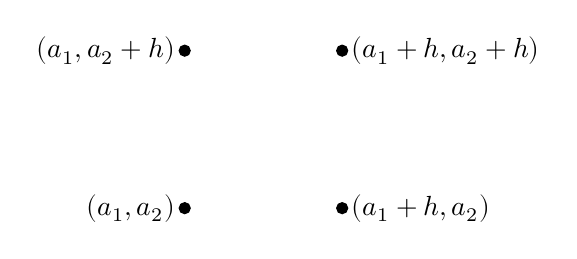
\begin{tikzpicture}[scale = 1]
      \draw [fill] (0, 0) circle (2pt);
      \draw [fill] (2, 0) circle (2pt);
      \draw [fill] (0, 2) circle (2pt);
      \draw [fill] (2, 2) circle (2pt);
      \node [left] at (0, 0) {\((a_1, a_2)\)};
      \node [right] at (2, 0) {\((a_1 + h, a_2)\)};
      \node [left] at (0, 2) {\((a_1, a_2 + h)\)};
      \node [right] at (2, 2) {\((a_1 + h, a_2 + h)\)};
    \end{tikzpicture}
  \end{center}
 Let
  \begin{align*}
    \Delta &= F(a_1 + h, a_2 + h) - F(a_1 + h, a_2) - F(a_1, a_2 + h) + F(a_1, a_2) \\
    A(t) &= F(a_1 + h, t) - F(a_1, t)
  \end{align*}
  so that
  \begin{align*}
    \Delta &= A(a_2 + h) - A(a_2) \\
    A'(t) &= \D_2 F|_{(a_1 + h, t)} - \D_2 F|_{(a_1, t)}
  \end{align*}
  By Mean Value Theorem applied to \(A\), we see that
  \begin{align*}
    \Delta &= h \cdot A'(x_2(h)) \\
    \intertext{where \(x_2(h) \in [a_2, a_2 + h]\)}
           &= h \cdot \left( \D_2 F|_{(a_1 + h, x_2(h))} - \D_2 F|_{(a_1, x_2(h))} \right) \\
           &= h \cdot (B(a_1 + h) - B(a_1)) \\
    \intertext{where}
    B(s) &= \D_2 F|_{(s, x_2(h))} \\
    B'(s) &= \D_1 (\D_2 F)|_{(s, x_2(h))} = \D_{21} F|_{(s, x_2(h))} \\
    \intertext{so by Mean Value Theorem again}
           &= h^2 \D_{21} F|_{(x_1(h), x_2(h))}
  \end{align*}

  In summary, \(\Delta = h^2 \D_{21} F|_{x_1(h), x_2(h)}\) so
  \[
    \lim_{h \to 0} \frac{\Delta}{h^2} = \lim_{h \to 0} D_{21} F(x_1(h), x_2(h))
  \]
  where \(x_1(h) \in [a_1, a_1 + h], x_2(h) \in [a_2, a_2 + h]\). Thus we know
  \[
    \lim_{h \to 0} (x_1(h), x_2(h)) = (a_1, a_2).
  \]
  Since \(F \in C^2(U)\), \(\D_{21} F\) is continuous so
  \[
    \lim_{h \to 0} \D_{21} F(x_1(h), x_2(h)) = \D_{21} F|_a = \lim_{h \to 0} \frac{\Delta}{h^2}.
  \]
\end{proof}

\begin{proof}[Proof of \nameref{thm:symmetry of mixed partials}]
  This should be almost apparent from the symmetry of the expression on RHS above. Let \(G(x_1, x_2) = F((x_2, x_1)\). Then
  \begin{align*}
    \D_{12} F|_{(a_1, a_2)} &= \D_{21} G|_{(a_2, a_2)} \\
                            &= \lim_{h \to 0} \frac{1}{h^2} \left( G(a_1 + h, a_2 + h) - G(a_1, a_2 + h) - G(a_1 + h, a_2) + G(a_1, a_2) \right) \\
                            &= \lim_{h \to 0} \frac{1}{h^2} \left( F(a_1 + h, a_2 + h) - F(a_1 + h, a_2) - F(a_1, a_2 + h) + F(a_1, a_2) \right) \\
                            &= \D_{21} F|_{(a_1, a_2)}
 \end{align*}
\end{proof}

\begin{corollary}
  Suppose \(U \subseteq \R^n\) is open, \(F \in C^2(\R^n)\). Then
  \[
    D_{ij} F|_a = D_{ji} F|_a
  \]
  for all \(1 \leq i \leq j \leq n\) and all \(a \in U\).
\end{corollary}

\begin{proof}
  Apply \nameref{thm:symmetry of mixed partials} to
  \[
    G(x_1, x_2) = F(a_1, \dots, a_{i - 1}, x_1, a_{i + 1}, \dots, a_{j - 1}, x_2, a_{j + 1}, \dots, a_n).
  \]
\end{proof}

To summarise, if \(F \in C^2(U)\) then the Hessian matrix
\[
  H|_a = \left( D_{ij} F|_a \right)
\]
is symmetric. We have proved that the second derivative is given by
\begin{align*}
  \D^2 F|_a: \R^n \times \R^n &\to \R \\
  (v, w) &\mapsto v^T H|_a w
\end{align*}
so \(\D^2 F|_a\) is a \emph{symmetric bilinear form}:
\[
  \D^2 F|_a(v, w) = \D^2 F|_a(w, v).
\]

We could rephrase our theory for second derivatives developed so far using the language of linear maps, which gives an alternative descriptoin from a slightly different point: if \(f: U \to \R^m\) is \(C^2\), then
\begin{align*}
  \D f: U &\to L(\R^n, \R^m) \cong \matrixring_{m, n}(\R) \cong \R^{mn} \\
  \D (\D f)|_a &\in L(\R^n, L(\R^n, \R^m)).
\end{align*}
i.e.\ if \(w \in \R^n, v \in \R^n\),
\[
  \D (\D f)|_a (w) \in L(\R^n, \R^m).
\]
Define a function
\[
  B(v, w) = (\D( \D f)|_a (w))(v)
\]
which is a clearly bilinear map \(\R^n \times \R^n \to \R^m\) and it is not hard too see that
\[
  B(v, w) = \D^2 f|_a (v, w)
\]
as we defined it.

\subsubsection{Third and Higher Derivatives}

\begin{definition}[\(C^k\) space]\index{Ck@\(C^k\)}
  \(F: U \to \R\) is \(C^k\) if the partial derivatives \(\D_i F\) are \(C^{k - 1}\) for all \(1 \leq i \leq n\).

  If \(F \in C^k(U)\), define the \(k\)th derivative
  \begin{align*}
    \D^k F|_a: (\R^n)^k &\to \R \\
    (v_1, \dots, v_k) &\mapsto \D( \D^{k - 1} F(v_1, \dots v_{k - 1}))|_a (v_k)
  \end{align*}
  which is a \emph{symmetric multilinear form}.
\end{definition}

\begin{note}
  The above definition also applies to \(F: U \to \R^m\).
\end{note}

\subsection{Taylor's Formula}

Let \(U \subseteq \R^n\) be convex and open, \(F \in C^k(U)\) and \(x_0, x_0 + v \in U\). Define
\[
  f(t) = F(x_0 + tv).
\]
Note that \(f: [0, 1] \to \R\).

\begin{proposition}
  \(f\) is \(k\)-times differentiable and
  \[
    f^{(k)}(t) = \D^k F|_{x_0 + tv} (v, \dots, v).
  \]
\end{proposition}

\begin{proof}
  If \(G \in C^k(U)\), \(g(t) = G(x_0 + tv)\) then
  \begin{equation}
    \label{eqn:taylor}
    g'(t) = \D_v G|_{x_0 + v} = \D G|_{x_0 + v} (v).
    \tag{\(\ast\)}
  \end{equation}
  Proof is by induction on \(k\). \(k = 1\) is \eqref{eqn:taylor} with \(G = F\). In general define
  \begin{align*}
    h(t) &= f^{(k - 1)}(t) \\
         &= \D^{k - 1} F|_{x_0 + tv} (v, \dots, v) \\
         &= H(x_0 + tv)
  \end{align*}
  where \(H(x) = \D^{k - 1} F|_x(v, \dots, v)\).

  Applying \eqref{eqn:taylor} to \(h\) gives
  \begin{align*}
    f^{(k)}(t) &= h'(t) \\
               &= \D H|_{x_0 + tv}(v) \\
               &= \D( \D^{k - 1} F(v, \dots, v))(v) \\
               &= \D^k F(v, \dots, v)
  \end{align*}
\end{proof}

\begin{corollary}[Multivariable Taylor's Formula]
  If \(U\) is open and convex, \(x_0, x_0 + v \in U\) and \(F \in C^k(U)\) then
  \[
    F(x_0 + v) = \sum_{i = 0}^{k - 1} \frac{1}{i!} \D^i F|_{x_0} (v, \dots, v) + \frac{1}{k!} \D^k F|_{x + tv}(v, \dots, v)
  \]
  for some \(t \in [0, 1]\).
\end{corollary}

\begin{proof}
  This seems like a horrible mess but, like many other things we have encountered in this course, its nothing more than ideas from IA Analysis I applied new (actually gneralised from old) definitions. Define
  \[
    f(t) = F(x_0 + tv).
  \]
  Then the single variable Taylor's formula says that
  \[
    f(1) = \sum_{i = 0}^{k - 1} \frac{1}{i!} f^{(i)}(0) 1^i + \frac{1}{k!} f^{(k)}(t)1^k
  \]
  for some \(t \in [0, 1]\). Subsituting the formula for \(f^{(i)}\) as in the proposition above gives the result required.
\end{proof}

\subsection{Speed \& Distance}


Well the title says all. This a bewildering section that doesn't seem to go anywhere or belong to any part of this course. Nevertheless it is required by the faculty.\footnote{``All right let's go ahead and get started.''}

All norms are Euclidean norms in this section since we require inner product.

\begin{lemma}
  If \(\alpha: \R \to \R^n\) is \(C^1\) then
  \[
    \frac{d}{dt} \norm{\alpha(t)} \leq \norm{\alpha'(t)}.
  \]
\end{lemma}

\begin{proof}
  \(\norm{\alpha(t)} = (\alpha \cdot \alpha)^{1/2}\) so
  \begin{align*}
    \frac{d}{dt}(\alpha \cdot \alpha)^{1/2} &= \frac{1}{2} (\alpha \cdot \alpha)^{-1/2} (2\alpha' \cdot \alpha) \\
                                            &= \frac{\alpha' \cdot \alpha}{(\alpha \cdot \alpha)^{1/2}} \\
                                            &\leq \frac{\norm{\alpha'} \norm \alpha}{\norm \alpha} \\
                                            &= \norm{\alpha'}
  \end{align*}
  by Cauchy-Schwarz.
\end{proof}

\begin{corollary}
  \label{cor:distance and displacement}
  If \(\gamma: \R \to \R^n\) is continuous then
  \[
    \norm*{\int_{0}^{1} \gamma(t) dt} \leq \int_{0}^{1} \norm*{\gamma(t)} dt
  \]
\end{corollary}

\begin{note}
  If \(\gamma(t) = v(t)\) is the velocity then this says displacement is smaller than distance on the odometer.
\end{note}

\begin{proof}
  Let \(\alpha(s) = \int_{0}^{s} \gamma(t) dt\). Then by the lemma
  \[
    \frac{d}{ds} \norm{\alpha(s)} \leq \norm{\alpha'(s)} = \norm{\gamma(s)}
  \]
  where the equality comes from Fundamental Theorem of Calculus. Let \(\beta(s) = \int_{0}^{s} \norm{\gamma(t)} dt\) then \(\beta'(s) = \norm{\gamma(s)}\).

  Since \(\norm{\alpha(0)} = 0 \beta(0)\) and
  \[
    \frac{d}{ds} \norm{\alpha(s)} \leq \norm{\gamma(s)} = \frac{d}{ds} B(s),
  \]
  \[
    \norm{\alpha(s)} \leq \beta(s)
  \]
  for all \(s \geq 0\). Take \(s = 1\) to get the result required.
\end{proof}

And that marks the end of this vestigial section.

\section{Metric Spaces}

In this chapter we take a short break from differential calculus (but don't forget them! We will need them shortly after).

\subsection{Definitions}

\begin{definition}[Metric space]\index{metric}
  A \emph{metric space} is a set \(X\) with a distance function \(D: X \times X \to \R\) satisfying
  \begin{enumerate}
  \item positivity: \(d(x, y) \geq 0, d(x, y) = 0\) if and only if \(x = y\).
  \item symmetry: \(d(x, y) = d(y, x)\) for all \(x, y \in X\).
  \item triangle inequality: \(d(x, z) \leq d(x, y) + d(y, z)\) for all \(x, y, z \in X\).
  \end{enumerate}
\end{definition}

\begin{eg}\leavevmode
  \begin{enumerate}
  \item A normed space \((V, \norm \cdot)\) is a metric space with
    \[
      d(v, w) = \norm{v - w}.
    \]

    \begin{proof}\leavevmode
      \begin{enumerate}
      \item \(d(v, w) = \norm{v - w} \geq 0\) and \(d(v, w) = 0\) if and only if \(\norm{v, w} = 0\) if and only if \(v - w = 0\) if and only if \(v = w\).
      \item \(d(v, w) = \norm{v - w} = \norm{(-1)(w - v)} = |-1| \cdot \norm{w - v} = d(w, v)\).
      \item \(d(v_1, v_3) = \norm{v_1 - v_3} \leq \norm{v_1 - v_2} + \norm{v_2 - v_3} = d(v_1, v_2) + d(v_2, v_3)\).
      \end{enumerate}
    \end{proof}
  \item If \((x, d)\) is a metric space and \(Y \subseteq X\) then \((Y, d|_{Y \times Y})\) is metric space. We say \(Y\) is a \emph{subspace} of \(X\).
  \item For any set \(X\), let
    \[
      d(x, y) =
      \begin{cases}
        1 & x = y \\
        0 & x \neq y
      \end{cases}
    \]
    which is the \emph{discrete metric}.
  \end{enumerate}
\end{eg}

Most of the definitions and theorems we gave about subsets of normed spaces apply equally well to metric spaces by replacing \(\norm{v - w}\) with \(d(v, w)\). Actually metric is a more fundamental concept than norm: every norm induces a metric as outlined above but not vice versa. This means that we could have organised the contents in a more structured and formal way by introducing metric spaces and its properties upfront and subsequently allowing normed spaces to inherit these properties. However, we choose not to do so since

\begin{enumerate}
\item for most of the course up to this point, properties of metric spaces are in a sense add complexity but not richness to our theory because we work with \(\R^n\) and function spaces, which come with a normed structure. Differential calculus in high dimension is already hard and we don't want to make things more complicated.
\item in fact, we don't use metric properties until the last chapter. It might be better to give an ad hoc definition here lest one forget if we do it at the very beginning.
\end{enumerate}

That is enough digression about the structure of the course. As promised, here are some definitions and results that generalise easily those from normed space. You should find them at this point very familiar (and more so if you've taken IB Metric and Topological Spaces).

\begin{definition}[Convergence]\index{convergence}
  A sequence \((x_n)\) in \(X\) \emph{converges} to \(x \in X\) if for every \(\varepsilon > 0\), there exists \(N\) such that \(d(x_n, x) < \varepsilon\) whenever \(n > N\).
\end{definition}

\begin{definition}[Continuity]\index{continuity}
  If \((X, d_x)\) and \((Y, d_Y)\) are metric spaces, \(f: X \to Y\) is continuous if \((f(x_n)) \to f(x)\) with respect to \(d_Y\) whenever \((x_n) \to x \in X\) with respect to \(d_X\).
\end{definition}

\begin{proposition}[Alternate characterisation of continuity]
  \(f\) is continuous if and only if for every \(\varepsilon > 0\) and \(x \in X\), there exists \(\delta > 0\) such that \(d(f(x'), f(x)) < \varepsilon\) whenever \(d(x', x) < \delta\).
\end{proposition}

\begin{definition}[Open ball]
  The set 
  \[
    B_r(x) = \{x' \in X: d(x', x) < r\}
  \]
  is the \emph{open ball} of radius \(r\) centred at \(x\).
\end{definition}

\begin{definition}[Closed ball]
 The set
   \[
     B_r(x) = \{x' \in X: d(x', x) \leq r\}
   \]
   is the \emph{closed ball} of radius \(r\) centred at \(x\).
\end{definition}

\begin{definition}[Open subset]\index{open subset}
  \(U \subseteq X\) is an \emph{open} subset of \(X\) if for every \(x \in U\), there exists \(\varepsilon > 0\) such that \(B_\varepsilon(x) \subseteq U\).
\end{definition}

\begin{proposition}
  If \(f: X \to Y\) is continuous and \(U \subseteq Y\) is open then
  \[
    f^{-1}(U) \subseteq X
  \]
  is open.
\end{proposition}

We have stressed this before but in case one has forgotten,

\begin{note}
  Being open (and closed) is a property of a \emph{subset}, not a space.
\end{note}

\begin{eg}
  Let \(X = \R\) with metric \(d(x, y) = |x - y|\). Then \([0, \frac{1}{2})\) is not an open subset of \(X\). If \(Y = [0, 1] \subseteq X\) with the subspace metric then \([0, \frac{1}{2})\) is an open subset of \(Y\).
\end{eg}

\begin{definition}[Closed subset]\index{closed subset}
  \(C\) is a \emph{closed subset} of \(X\) if \(X \setminus C\) is an open subset.
\end{definition}

\begin{proposition}
  \(C \subseteq X\) is closed if and only if whenever \((x_n) \to x\) in \(X\) and \(x_n\)'s are all in \(C\) then \(x \in C\) as well.
\end{proposition}

\begin{definition}[Cauchy sequence]\index{Cauchy}
  A sequence \((x_n)\) in \(X\) is \emph{Cauchy} if for every \(\varepsilon > 0\) there exists \(N\) such that \(d(x_n, x_m) < \varepsilon\) whenever \(n, m \geq N\).
\end{definition}

\begin{definition}[Completeness]\index{completeness}
  \(X\) is \emph{complete} if whenever \((x_n)\) is a Cauchy sequence in \(X\), there exists \(x \in X\) such that \((x_n) \to x\).
\end{definition}

\begin{proposition}
  Suppose \(X\) is a complete metric space and \(C \subseteq X\) is closed. Then \(C\) with the subspace metric is also complete.
\end{proposition}

\begin{proof}
  Suppose \((x_n)\) is a Cauchy sequence in \(C\). Then \((x_n)\) is also a Cauchy sequence in \(X\). Since \(X\) is complete there exists \(x \in X\) such that \((x_n) \to x\). Since \(C \subseteq X\) is closed \(x \in C\) so \(C\) is complete.
\end{proof}

\begin{joke}
  This is a story about John Conway. Before he moved to the U.S. he was a professor here in Cambridge. He was a very unusual guy and liked playing games. His office was full of toys, such as balls to study sphere packing. In fact he had two offices full of toys: the first one was filled up so he was given a second one.

  One day he had his attic repainted. When the painters finished, they left behind this long roll of paper and an enormous pair of shears. They came back and collect hte shears but not didn't bother the paper.

  Back then Conway was interested in finite simple group. Around that time someone suspected a new finite simple group and Conway proposed a way to build it. Other group theorists told Conway that, well, if you want to prove it then just write down the character table (which is enormous). But he was too busy to get started.

  Just about then he thought it would a really good idea to use the paper at hand to do this. He cover the floor of attic with paper and started working on the character table. And indeed he found it, so now we have a finite simple group (actually three) called Conway group.\footnote{Moral of the story: sometimes you just need a really big piece of paper!}
\end{joke}

\subsection{Lipschitz Maps}

Suppose \((X, d_X)\) and \((Y, d_Y)\) are metric spaces.

\begin{definition}[Lipschitz map]\index{Lipschitz map}
  \(f: X \to Y\) is \emph{\(K\)-Lipschitz}, where \(K \in \R, K > 0\), if for every \(x, x' \in X\),
  \[
    d_Y(f(x), f(x')) \leq K d_X(x, x').
  \]

  Say \(f\) is \emph{Lipschitz} if it is \(K\)-Lipschitz for some \(K\).
\end{definition}

\begin{eg}\leavevmode
  \begin{enumerate}
  \item If \(f\) is Lipschitz then it is uniformly continuous:

    \begin{proof}
      Suppose \(f\) is \(K\)-Lipschitz. Given \(\varepsilon > 0\), \(d(f(x), f(x')) \leq K d(x, x') < \varepsilon\) whenever \(d(x, x') < \varepsilon/K\).
    \end{proof}
  \item Suppose \(U \subseteq \R^n\) is open, \(F \in C^1(U)\). If \(K = \cl B_r(x_0) \subseteq U\) then \(F|_K\) is Lipschitz:

    \begin{proof}
      The function
      \begin{align*}
        U & \to \R^n \to \R \\
        x &\mapsto \gradient F|_x \mapsto \norm{\gradient F|_x}
      \end{align*}
      is continuous. \(K\) is closed and bounded and thus compact. Thus by Maximum Value Theorem there exists \(M\) such that \(\norm{\gradient F|_x} \leq M\) for all \(x \in K\). \(K = \cl B_r(x_0)\) is convex so by Mean Value Inequality
      \[
        |F(x) - F(x')| \leq M \norm{x - x'}
      \]
      so \(f\) is \(M\)-Lipschitz.
    \end{proof}
  \item If \(f: X \to Y\) is \(K_1\)-Lipschitz, \(g: Y \to Z\) is \(K_2\)-Lipschitz then \(g \compose f\) is \(K_1K_2\)-Lipschitz:

    \begin{proof}
      \begin{align*}
        d(g(f(x)), g(f(x'))) &\leq K_2 d(f(x), f(x')) \\
                            &\leq K_2K_2 d(x, x')
      \end{align*}
    \end{proof}
  \item Consequently, composition of Lipschitz maps is Lipschitz.
  \item If \(\norm \cdot\) and \(\norm \cdot'\) are two norms on \(V\). Then they are Lipschitz equivalent if and only if the maps
    \begin{align*}
      \id: (V, \norm \cdot) &\to (V, \norm \cdot') \\
      \id: (V, \norm \cdot') &\to (V, \norm \cdot)
    \end{align*}
    are both Lipschitz.
  \end{enumerate}
\end{eg}

\subsubsection{Operator Norm}

\begin{definition}[Operator norm]\index{operator norm}
  Let \(V\) and \(W\) be normed spaces. Given \(L \in L(V, W)\), the \emph{operator norm} is
  \[
    \nop L = \sup_{v \in V\setminus \{0\}} \frac{\norm{L(v)}_W}{\norm v_V} = \sup_{v \in V \setminus \{0\}} \norm*{ L\left( \frac{v}{\norm v} \right)}
    \]
\end{definition}

\begin{remark}
  If \(V\) and \(W\) are finite-dimensional, \(L \in L(V, W)\) is continuous and \(S(V) = \{v \in V: \norm v = 1\}\) is compact. By the Maximum Value Theorem,
  \[
    \sup_{v \in S(V)} \norm{L(v)} = \max_{v \in S(V)} \norm{L(v)}.
  \]
  so we can replace \(\sup\) with \(max\) in the definition.
\end{remark}

Observe that if \(v \in V\) then \(\norm{L(v)} \leq \nop L \cdot \norm v\).

We call something a norm without checking whether it is a norm so we had better do it now:

\begin{proposition}
  \(\nop \cdot\) is a norm on \(L(V, W)\).
\end{proposition}

\begin{proof}\leavevmode
  Example sheet.
\end{proof}

Form here on let \(V = (\R^n, \norm \cdot_2)\) and \(W = (\R^m, \norm \cdot_2)\).

\begin{proposition}
  Suppose \(U \subseteq \R^n\) is open and convex, \(f: U \to \R^m\) is differentiable and \(\nop{\D f|_x} \leq M\) for all \(x \in U\). Then \(f\) is \(M\)-Lipschitz.
\end{proposition}

\begin{proof}
  This is nothing more than a corollary of Mean Value Inequality.

  Given \(x_0, x_1 \in U\), define
  \begin{align*}
    x: [0, 1] &\to U \\
    t &\mapsto (1 - t)x_0 + t x_1 \\
    \gamma: [0, 1] &\to \R^m \\
    t &\mapsto f(x(t))
  \end{align*}
  By \Cref{cor:distance and displacement},
  \[
    \norm*{\int_{0}^{1} \gamma'(t) dt} \leq \int_{0}^{1} \norm{\gamma'(t)} dt
  \]
  By Fundamental Theorem of Calculus, LHS is
  \[
    \norm*{\int_{0}^{1} \gamma'(t) dt} = \norm{\gamma(1) - \gamma(0)} = \norm{f(x_1) - f(x_0)},
  \]
  and by chain rule the integrand on RHS is
  \[
    \norm{\gamma'(t)} = \norm*{ \D f|_{x(t)}(x'(t))} \leq \norm{\D f|_{x(t)}} \cdot \norm{x'(t)} \leq M \norm{x_1 - x_0}.
  \]
  Thus putting everyting together we get
  \[
    \norm{f(x_1) - f(x_0)} \leq M \norm{x_1 - x_0}.
  \]
\end{proof}

\subsection{Contraction Mapping Theorem}

In this section we will learn a new way to solve equations.

\begin{definition}[Contraction map]\index{contraction}
  Let \(X\) be a metric space. \(f: X \to X\) is a \emph{contraction map} if it is \(K\)-Lipschitz for some \(K < 1\), i.e.
  \[
    d(f(x), f(x')) \leq K d(x, x').
  \]
\end{definition}

Intuitively, \(f\) shrinks distances, ergo the name.

\begin{definition}[Fixed point]
  \(x \in X\) is a \emph{fixed point} of \(f: X \to X\) if \(f(x) = x\).
\end{definition}

\begin{theorem}[Contraction Mapping Theorem]
  Suppose \(X\) is a \emph{complete} metric space. If \(f: X \to X\) is a contraction map then \(f\) has a unique fixed point.
\end{theorem}

\begin{proof}
  Since \(f\) is a contraction, there is some \(K < 1\) such that
  \[
    d(f(x), f(x')) \leq K d(x, x').
  \]

  We prove the uniqueness part first since it is short. Suppose \(x\) and \(x'\) are both fixed points of \(f\), then
  \[
    d(x, x') = d(f(x), f(x')) \leq K d(x, x')
  \]
  where \(K < 1\). The only way for this to hold is \(d(x, x') = 0\), i.e.\ \(x = x'\).

  Next we prove the more interesting part about existence. Heuristically, completeness appears in our hypothesis although it is not in any part of the definition of a contraction map or fixed point, so we better find a Cauchy sequence to which we can apply the condition. Pick \(x_0 \in X\) and inductively define
  \[
    x_{n + 1} = f(x_n) = f^{n + 1}(x_0).
  \]
  Observe that
  \[
    d(x_n, x_{n + 1}) = d(f(x_{n - 1}), f(x_n)) \leq K d(x_{n - 1}, x_n)
  \]
  so by induction we see that
  \[
    d(x_n, x_{n - 1}) \leq K^n d(x_0, x_1) = K^n R
  \]
  where \(R = d(x_0, x_1)\). Claim \((x_n)\) is Cauchy:

  \begin{proof}
    \begin{align*}
      d(x_n, x_{n + r}) &\leq d(x_n, x_{n + 1}) + d(x_{n + 1}, x_{n + 2}) + \dots + d(x_{n + r -1}, x_{n + r}) \\
                        &\leq K^n R + K^{n + 1} R + \dots + K^{n + r - 1} R \\
                        &= K^n R \frac{1 - K^r}{1 - K} \\
                        &\leq K^n R \frac{1}{1 - K}
    \end{align*}
    As \(K < 1\),
    \[
      \lim_{n \to \infty} \frac{K^n R}{1 - K} = 0.
    \]

    Given \(\varepsilon > 0\), pick \(N\) such that \(\frac{K^nR}{1 - K} < \varepsilon\) whenever \(n \geq N\). Then for \(m \geq n \geq N\),
    \[
      d(x_n, x_m) \leq \frac{K^nR}{1 - K} < \varepsilon
    \]
    so \((x_n)\) is Cauchy.
  \end{proof}

  Since \(X\) is complete, there exists \(x \in X\) such that \((x_n) \to x\). \(f\) is Lipschitz so it is continuous so \((f(x_n)) \to f(x)\), i.e.
  \((x_{n + 1}) \to f(x)\). But \((x_{n + 1}) \to x\) so by uniqueness of limits in metric space \(f(x) = x\), i.e.\ \(x\) is a fixed point of \(f\).
\end{proof}


\begin{remark}
  How does this help us solve equations? The theorem says that the equation \(f(x) = x\) has a unique solution and the proof shows that we can approximate the fixed point by starting with \(x_0 \in X\) and repeatedly applying \(f\).
\end{remark}

In practice, not every map is contraction so we often have to restrict the domain of \(f\) in order to get a contraction map.

\begin{eg}[Finding square roots using iteration]
  An elementary method to find the square root of a non-negative number \(n\) is to let
  \begin{align*}
    f: (0, \infty) &\to (0, \infty) \\
    x &\mapsto \frac{1}{2} \left( x + \frac{n}{x} \right)
  \end{align*}
  and iterate \(f\).

  Why does this work? We are essentially finding a fixed point of \(f\). But then \(x = f(x) = \frac{1}{2}(x + n/x)\) so \(x^2 = n\). Therefore the fixed point of \(f\) is precisely \(\sqrt n\).

  That seems promising. Now we are left to show \(f\) is a contraction:
  \[
    |f(x) - f(y)| = \frac{1}{2} \left|x + \frac{n}{x} - y - \frac{n}{y} \right| = \frac{1}{2} |x - y| \cdot \left|1 - \frac{n}{xy} \right|.
  \]
  Unfortunately, this means that if \(x\) and \(y\) are small \(f\) is definitely not a contraction. To fix this, we restrict \(f\) to \(I_K = [\sqrt n /K, K \sqrt n]\). Then \(f(I_K) \subseteq I_K\) and if we choose \(K = \sqrt 2\), for example, then
  \[
    \left|1 - \frac{n}{xy} \right| \leq |1 - 2| = 1
  \]
  so
  \[
    |f(x) - f(y)| \leq \frac{1}{2} |x - y| \cdot 1 = \frac{1}{2} |x - y|
  \]
  for \(x, y \in I_K\) so \(f|_{I_{\sqrt 2}}\) is a contraction map. Therefore if I start with \(x_0 \in I_{\sqrt 2}\) and iterate it will converge to \(\sqrt n\).
\end{eg}

\printindex
\end{document}
